\documentclass[11pt,twoside,a4paper]{article}

\usepackage{a4wide,amsmath,amssymb}
\usepackage[school, simplified]{pgf-umlcd}
\usetikzlibrary{calc}
\usetikzlibrary{positioning}

% Mann will direkt Umlaute eingeben können statt \"a, \"o, \"u usw.
% Entweder:
\usepackage[utf8]{inputenc}
% oder:
%\usepackage{umlaut}
\usepackage[german]{babel}

\usepackage[style=numeric]{biblatex}
\addbibresource{grr.bib}

\usepackage{textcomp}
\usepackage{graphicx}
\usepackage{subcaption}

\usepackage{hyperref}

\usepackage{tikz}
\usepackage{background}
%uncomment next line to remove "Draft" watermark
%\backgroundsetup{contents={}}


% Trennvorschl"age (in {} einfuegen, wenn nicht automatisch getrennt wird:
% z.B. Authen-ti-ka-tions-sys-tem)
%\hyphenation{}

%\hyphenation{min-des-tens}
%\hyphenation{Kol-li-sions-er-ken-nung}


%-------------------------- Formatsachen --------------------------%

% Bild-, Tabellenunterschriften veraendern:
% Nummer fett, kleinerer Text fuer Bildunterschrift
%\usepackage[bf,small]{caption}


%\usepackage{mathpazo}  % -- Palatino als Zeichensatz -- einfach diese
					   % Zeile auskommentieren, falls nicht installiert
%\usepackage{mathptmx}  % -- Times als Zeichensatz

% Zum Unterscheiden von Entwurfs- und endgueltiger Fassung
%\usepackage{draftcopy}
%\draftcopySetGrey{0.90}   %   90% = sehr helles Grau
%\draftcopyName{ENTWURF}{155}   % statt ``DRAFT''
%\draftcopySetScale{1}

%--------------- Zeilen- und Absatzabstaende ----------------------%
%\setlength{\parindent}{0em}
%\setlength{\parskip}{\medskipamount}    % Abstand zwischen Abs"atzen

\newcommand{\obj}{\operatorname{OBJ}}
\newcommand{\pos}{\operatorname{pos}}
\newcommand{\rot}{\operatorname{rot}}
\newcommand{\gridsize}{s_{\mathit{grid}}}
\newcommand{\tometer}{\mathit{meter}}
\newcommand{\calAABB}{\mathcal{AABB}}
\newcommand{\AABB}{\mathit{AABB}}
\newcommand{\qb}{\operatorname{QB}}

\begin{document}

\title{HSP-Projektarbeit im Master Informatik \\
\small Echtzeitsynchronisation von Simulationen mit Fokus auf die Verwendung in Videospielen}
\author{Robert Graf, Lukas Hermann\\
%  (\texttt{fridolw@in.tum.de})\\[5mm]
%  Seminar "`Internetrouting"' , \\
  Ostbayerische Technische Hochschule Regensburg\\
  \\
  Projektbetreuung: Prof. Dr. Markus Kucera
}
  
\date{WS\, 2019/2020 (Version vom \today)}

\maketitle

\newpage
\tableofcontents
\newpage


\abstract{Das Projekt umfasst die Erstellung, bzw.~Umwandlung, einer 3D-Simulation mit dem Fokus auf die Umsetzung einer Echtzeitsynchronisierung besagter Simulation zwischen zwei Simulationsinstanzen auf verschiedenen Rechenmaschinen, bzw.~Prozessen. Dabei werden sowohl Techniken der verlustarmen Implementierung der Synchronisation erschlossen, als auch benötigte Anforderungen und Designaspekte ermittelt.}


\section{Einleitung}


\subsection{Kontext und Motivation}
Eine Echtzeitsynchronisation einer Simulation auf mehrere über Netzwerk verbundene Rechenmaschinen soll die Äquivalenz der Simulationszustände auf allen beteiligten Maschinen zum selben, oder annehmbar ähnlichen Zeitpunkt gewährleisten.\\
Das Ziel ist die Kollaborative Verwendung der Simulation. 
Dazu zählen sowohl die Anzeige von Simulationsinhalten, als auch
die benutzerdefinierte Veränderung dieser. 
Die Synchronisation der Simulationszustände beinhaltet demnach die rechtzeitige Synchronisation der Änderungen.

Nach dieser Definition oder nach dessen Teilen, finden wir Echtzeitsynchronisation in industriellen Anwendungen wieder. Zum Beispiel kann im Bereich der Robotik der rechtzeitige Informationsfluss zwischen Steuergeräten und Sensoren als Echtzeitsynchronisation angesehen werden.
%%TODO cite example
Das wohl ähnlichste Anwendungsbeispiel im Kontext dieser Arbeit lässt sich im Bereich der Videospiele, oder Bedienersimulationen finden, wo ein echtzeitsynchronisierter Simulationsstatus auf mehreren Maschinen lokal angezeigt werden muss, Bediener jedoch auch selbst Einfluss auf die Simulationsinhalte nehmen können.\\
In diesem Projekt wird auf einer bestehenden Codebasis einer Simulation, welche nicht unter Einbezug von Synchronisationsgedanken entwickelt wurde, eine solche umgesetzt. Dabei soll eine Echtzeitsynchronisation zwischen mehreren Rechenmaschinen über eine Internetverbindung mit 100\,KByte/s Bandbreite erreicht werden.
Das letztendliche Ziel ist die möglichst unmerkliche Synchronisierung zweier Simulationszustände und deren Anzeige, d.h. die Reduzierung von Seiteneffekten durch Latenz.\\
Im Laufe der Arbeit werden Kernaspekte zur Synchronisation, aber auch zum benötigten Softwaredesign ermittelt, um synchrone Applikationen umzusetzen. Durch den Status-Quo der übernommenen Codebasis werden durch die Überarbeitung dort gemachte Fehler in diesen Aspekten erkenntlich.

\subsection{Beschreibung der konkreten Simulationsanwendung}
Die verwendete Simulationsanwendung ist ein rudimentäres 3D-Shooter-Videospiel. Ein Spieler kann dabei in einem Terrain auf Gegnerfiguren schießen, diese beschädigen und wird dabei durch Punkte entlohnt. Diese einfache Anwendung hält bereits alle Kernaspekte einer Simulation im Kontext dieser Arbeit inne:
\begin{itemize}
\item Die Simulation ist gezeitet und läuft in einer bestimmten Rate zur Realzeit. Diese Rate soll meist $1$ sein, bei der programmierte physikalische Vorgänge dieselbe Geschwindigkeit wie in der Realität annehmen. Die Simulation besitzt dadurch ihre eigene Simulationszeitbasis.
\item Verschiedene Arten von zu simulierenden Entitäten in einem Simulierten Raum (Gegner, Spielerfiguren, Projektile, Geräusche) mit unterschiedlichem Verhalten/unterschiedlicher Physik.
\item Interaktionen zwischen Entitäten (Kollisionen, Anti-Clipping)
\item Einflüsse durch Bediener/Spieler (Bewegung der Spielerfigur, Erzeugung von Projektilen)
\item Grafische Ausgabe in Echtzeit zu einer dreidimensionalen Perspektive
\end{itemize}

Die Simulation von Simulationsinhalten erfolgt in Schritten, in denen ein Inhalt von einem bestehenden Zustand auf einen Zustand zu fortgeschrittener Simulationszeit verändert wird. Ein solcher Zeitschritt wird als Tick bezeichnet (siehe Appendix \ref{sec:tick} oder vgl. Quelle \ref{tick}).\\
Die Anzeige der Simulation erfolgt durch Extrapolation des letzten bekannten Zustands der Simulationsinhalte. Die Anzeige führt dabei keine Änderungen auf den Simulationsinhalten durch. Wir bezeichnen den Prozess sowie sein Ergebnis als Frame (vgl. Appendix \ref{sec:tick}).
Die Framerate kann ungleich der Tickrate sein, um unabhängig von den Fähigkeiten des Anzeigesystems eine flüssiges Bild zu generieren. Da in einem Frame keine Simulationsinhalte geändert werden, sind die Simulationinhalte komplett unabhängig zur Anzeige.\\

In vielen kommerziellen Produkten in der Videospielbranche wird diese Trennung nicht sauber vollzogen.\\
Es folgen Inkonsistenzen in der Simulation in Abhängigkeit der Framerate.
(Beispiel in \glqq The Elder Scrolls V: Skyrim\grqq falsche physikalische Berechnungen auf Grund zu hoher Frameraten lernen Mammuts das Fliegen \cite{flying-fucking-mammoths})
Es existiert dort dann meist eine maximale Framerate.
Dieser Umstand scheint die Problematik mitzuführen, dass viele Videospielhersteller, vor allem im Konsolenbereich, Frameraten immer weiter nach unten limitieren, um ihre Produkte umzusetzen, was die Qualität erheblich senkt (Beispiele \cites{skyrim-physics-cap-and-fix, dark_souls-physics-cap-and-fix})
(entgegen der Meinung ihrer Marketingabteilungen, mit einer Menge negativer Presse, Beispiele \cites{morecinematic00, morecinematic01}
) und dazu führt dass Benutzer ihre u.U.~teure, fähige Hardware nicht ausnutzen können und sich mit schlechter Bildqualität zufrieden geben müssen.\\
Ein Umstand, der oft auf umständlichem Weg durch fähige Konsumenten selbstständig gelöst wird (vgl. \cites{skyrim-physics-cap-and-fix, dark_souls-physics-cap-and-fix})
Die Trennung von Physik und Grafik scheint eine grundsätzliche Designentscheidung zu sein, die in vielen kommerziell genutzten Engines fehlt.

Die beschriebene Anwendung funktioniert zu Beginn des Projektes lokal mit einem Benutzer. Es ist Ziel dieser Arbeit möglichst volle Funktionalität auf mehrere Benutzer, welche mit einer Netzwerkverbindung verbunden sind zu erweitern und dabei möglichst wenige negative Seiteneffekte zu erzeugen.

\subsection{Hergang}
Der Entwicklungsprozess in diesem Projekt umfasst das Erreichen bestimmter Meilensteine, die konstruktiv auf das Endziel hinführen sollen. Dieser Vorgang wird gewählt, um die Gesamtkomplexität des Endziels zu mitigieren. Durch die Abhängigkeit, die das Projekt vom Status quo des Vorprojektes hat, kann so dieses sukzessive an die hier gestellten Anforderungen angepasst werden.\\
Der Hergang lautet wie folgt:
\begin{enumerate}
\item Aufarbeitung des Status Quo\\
Umsetzung eines Designs im bestehenden Basisprojekt, das mit weiteren in diesem Projekt zu entwickelnden Features kompatibel ist.
\item Implementierung einer Fernbedienung\\
Fernbedienung als erstes netzwerkabhängiges Feature mit Einwegkommunikation, die keine Synchronisation benötigt.
\item Erneute Aufarbeitung
\item Implementierung der Echtzeitsynchronisation zwischen Simulationen\\
Auf zwei über Netzwerk verbundenen Maschinen wird jeweils eine Simulationsinstanz ausgeführt, deren Inhalte Synchronisiert werden.
\end{enumerate}



\section{Entwicklung der Softwarearchitektur einer synchronisierbaren Simulation}
Durch die Übernahme des Status-Quo eines bestehenden Projektes bestehen zunächst Probleme im Design der Applikation, die eine Umsetzung einer Synchronisation verhindern. Es ist daher eine Überarbeitung der generellen Architektur der Applikation gefordert, welche im Projekt sukzessive nach Bedarf per Meilenstein abgearbeitet wird.\\
Grundsätzlich wird angenommen, dass eine Echtzeitsynchronisation ständige Kommunikation zwischen beteiligten Knoten erfordert.
Information über aktiv simulierte Simulationsinhalte sollen so oft wie möglich wiederholt versendet werden, um die auf dem Remote verfügbare Information so aktuell wie möglich zu halten. Dabei müssen Einschränkungen der Übertragungsmedien und -methoden respektiert werden.\\
Die Last der Verarbeitung von Netzwerkkommunikation gegenüber der Last der aktiven lokalen Simulation von Inhalten wird als Vergleichsweise gering auf Grund der zur Verfügung stehenden Verbindung eingeschätzt. Relevante Parameter sind hier Latenz und Bandbreite.

\subsection{Übertragungsmethoden}
\label{sec:transmission_formats}
Perfekte Synchronität ist unter den Umständen von Latenz und der Möglichkeit der Einwirkung auf den Simulationszustand durch einen Bediener utopisch, da so unberechenbare Änderungen für den Simulationszustand existieren.
Zur Entwicklung einer möglichst optimalen Übertragung werden verschiedene Aspekte in die Überlegung mit einbezogen, wie die folgenden Abschnitte zeigen.

\subsubsection{Übertragungszweck}
Die Übertragung von Information im Rahmen der Synchronisation dient verschiedenen Teilzwecken.
Es wird zwischen Arten von Information unterschieden, für welche unterschiedliche Anforderungen für die Übertragung bestehen:
\begin{itemize}
\item Initialisierungsinformation\\
Beim initialen Verbindungsaufbau müssen Informationen ausgetauscht werden.
Derzeitig fallen nur organisatorische Informationen an, sämtliche die Simulation betreffenden Initialisierungsdaten, sowie Ressourcen, sind an beiden Enden der Verbindung statisch bekannt.
Zu den Aufgaben hier zählen:
\begin{itemize}
\item Filterung von Fremdverbindungen durch eine Begrüßung spezifisch zur Applikation
\item Identifikation von Servern und Clients (wir verzichten im Rahme dieser Arbeit auf Sicherheitsaspekte, wie z.B. saubere Authentifizierung, etc.)
\item Die Übermittlung der Adressierung von UDP-Sockeln der jeweiligen Knoten.
\end{itemize}
\item Echtzeitinformation\\
Information die sich ändert, insbesondere wenn die Änderung frequent ist.
Dies sind meist die Stati von Simulationsinhalten.
\end{itemize}

Außerdem kann für bestimmte Zwecke berechenbarer oder statischer Determinismus eingesetzt werden, um eine Übertragung komplett zu vermeiden.

\subsubsection{Transportschicht}
Es stehen zwei Protokolle der ISO-OSI Transportschicht zur Verfügung:
\begin{enumerate}
\item TCP, mit den relevanten Eigenschaften der Verbindungsorientiertheit, Erhaltung der Reihenfolge und Übertragungsversicherung als Abstraktion einer Stream-Datenstruktur\\
	Die Eigenschaften von TCP beinhalten für Echtzeitanwendungen jedoch gefährliche vorhersehbare Nachteile:\\
	Bei spontanem Paketverlust fallen Wartezeiten durch Sendewiederholung an, welche weiteren Informationserhalt über den TCP-Socket blockiert.\\
Ein Beispiel der unvorteilhaften Verwendung von TCP im Bereich von Videospielen ist das äußerst erfolgreiche und bekannte Spiel Minecraft von Mojang. Hier äußern sich Netzwerkverzögerungen (Lags) durch einen Stillstand der Spielabläufe, der sich über Sekunden ziehen kann und anschließendes Aufholen der Simulationszeit im Zeitraffer. Manch ein unverdientes Game Over kann daher von einem Gegner verursacht werden, der in der Zeit des Stillstandes Angriffe auf den Spieler im TCP-Puffer ansammelt, auf die der Spieler nicht reagieren kann. Dieser Umstand ist umso mehr Schade, wenn das verzögernde Paket zu dieser Zeit bereits schon, aufgrund von Echtzeitanforderungen, irrelevant ist, bzw. bereits ein aktuelleres im TCP-Puffer liegt.\\
Die Verwendung von TCP für echtzeitrelevante Information ist daher nur ratsam, wenn die zu übertragende Information die von TCP erhaltenen Eigenschaften von Reihenfolge und Übertragungssicherheit auch tatsächlich fordert. In diesem Fall muss ein Protokoll, welches diese Eigenschaften implementiert nicht im Rahmen von UDP selbst umgesetzt werden.\\
Durch seine Verbindungsorientiertheit bietet sich TCP ebenfalls für die Verbindungskontrolle an, da der Verbindungsstatus, z.B.~ bei abgebrochenen Verbindungen leicht erkannt werden kann. Des weiteren lassen sich auf der Basis einer TCP-Verbindung leicht eigene sequenzielle Protokolle implementieren, z.B. um eine Verbindung zweier Applikationen in der Applikationsschicht initial herzustellen.
\item UDP, maximale Größe von Einzelpaketen, sonst keine relevanten Anforderungen\\
	Im Videospielbereich sehen wir hauptsächlich UDP verwendet, höchstwahrscheinlich
	da die meisten Informationen im Rahmen der Echtzeitsynchronisation von Videospielen die unter TCP beschriebenen Eigenschaften nicht zwingend fordert.
\end{enumerate}

Im Folgenden werden diese Protokolle für hier enthaltenen Verwendungszwecke in Betracht gezogen und entsprechend ihrer Eigenschaften gewählt.

\subsubsection{Informationsformat}

Es werden prinzipiell zwei grundlegende Formate von temporärer Information für ein Übertragungsformat betrachtet.
\begin{enumerate}
\item Statusinformation\\
In der Simulation liegt die Information zu ihren Inhalten in Form von gezeiteten Stati vor, d.h. ein Zustand eines Simulationsinteresses zu einem bestimmten Zeitpunkt, sei dieser Real- oder Simulationszeit. \\
So ist ein Projektil z.B.~durch Position und Geschwindigkeit zu einem Simulationszeitpunkt dargestellt, welche nach entsprechenden physikalischen Gesetzen aktualisiert werden kann.\\
Die wohl interessanteste Eigenschaft von Statusinformation im Rahmen der Synchronisierung ist bei Mitführung des Zeitpunktes der Validität der Information die inhärente Redundanz bei wiederholter Übertragung durch simples überschreiben älterer Stati, welche die Übertragung sehr robust macht.
Das präferierte Übertragungsprotokoll für diese Art Information ist UDP, da es dessen Eigenschaftsprofil entspricht.
Wir erkennen jedoch auch, dass das Optimierungspotential von Synchronisationsprotokollen bei der Verwendung von roher Statusinformation beschränkt ist. Bei vielen Entitäten, oder bei komplexen Entitäten wird der benötigte Sendungsumfang unter Umständen zu groß.
Zum Beispiel werden beim Schießen einer Schrotflinte in der Simulation theoretisch zigfach Projektile frei, welche dann simuliert und synchronisiert werden sollen.
Unter der Verwendung von Statusinformation zur Synchronisation dieser Projektile steigt die Menge der zur Synchronisation versendeten Daten mindestens linear mit der Anzahl der Projektile.\\
Dieser Umstand kann nur durch eine abstraktere Behandlung von mehreren Projektilen in der Simulation, beispielsweise als Schwarm, oder eine abstraktere Übertragungsmethode abgeschwächt werden.
\item Aktualisierungsinformation\\
beschreibt die Änderung eines Zustands zu einem bestimmten Zeitpunkt. Diese umfassen meist codierte Anweisungen oder arithmetische Differenzen, welche auf den Status am Empfänger aufgerechnet werden.\\
Ein Problem mit Änderungsinformation besteht, wenn diese keine kommutativen und/oder assoziativen Eigenschaften beinhaltet und so sowohl die Übertragungsreihenfolge als auch die Übertragung selbst abgesichert sein muss, um die Äquivalenz des am Empfänger ermittelten Simulationsstatus sicherzustellen. In diesem Fall ist das präferierte Übertragungsprotokoll TCP, da dieses die so geforderten Eigenschaften mitbringt. Ist die Reihenfolge oder das Fehlen der Information am Empfänger allerdings nicht kritisch kann auch hierfür einfach UDP verwendet werden. Es ist jedoch hier essentiell eine Analyse zu vollziehen, da sonst zu synchronisierende Simulationsstati sich plötzlich und oft sogar unerkannt desynchronisieren können.

\end{enumerate}

\subsubsection{Generelle Präferenz}
Zur Übertragung von Initialisierungsinformation wird TCP verwendet, da die Erstellung eines sequenziellen Protokolls unter TCP einfacher erscheint und die enthaltene Übertragungssicherheit und Verbindungskontrolle für diesen Zweck ein erheblicher Vorteil ist.
Die Übertragung von Statusinformation via UDP wird unter den gegebenen Anforderungen auf Grund seiner Robustheit und Einfachheit als präferiert angesehen. Es wird zunächst versucht so viele Features wie möglich über diese Übertragungsstrategie abzubilden.\\
Die Verwendung von Änderungsinformation wird sich für andere Verwendungszwecke vorbehalten, hauptsächlich, da das Optimierungspotential hier höher scheint.


\subsection{Anmerkungen zur übernommenen Codebasis}
Durch die Hinzunahme von Echtzeitsynchronisationsfähigkeit als Anforderung an die Applikation werden im Design der übernommenen Codebasis schnell Verletzungen des \textit{Separation of Corcerns} Prinzips ersichtlich.\\
Das Fehlen von Anforderungen hinsichtlich mehrerer Benutzer und Fernsteuerung von Simulationsinhalten erlaubt in der übernommenen Codebasis für kurze Implementierungswege durch viele $1:1$ Beziehungen, welche sich hier weiter als kritisch erweisen. Belange(Concerns) sind über besagte $1:1$ Beziehungen dabei oft nicht sauber zum Vorteil der Erweiterbarkeit oder Umsetzung einer Synchronisation abgegrenzt. Komponenten sind unnötig engmaschig vernetzt, was Erweiterungen der $1:1$ Beziehungen auf Beziehungen mit mehreren Partnern, z.B. $1:n$, erschwert. 
Viele Basisaspekte der Simulationsengine werden daher komplett neu erdacht und designed, was den Hauptanteil der im Projekt aufgebrachten Zeit ausmacht.\\
Auch viele periphere Features werden von diesen Änderungen beeinflusst, oder es droht der Verlust des Features. Dabei werden oft Neurealisierungen des Features genauso Umfangreich wie seine Entfernung eingeschätzt.
Die konkreten vollzogenen Änderungen sind oft umfangreich und weitreichend, ihre Begründung allerdings komplex, detailreich und werden daher für diesen Bericht nicht als geeignet oder interessant eingeschätzt, zumal sie nichts zur konkreten Umsetzung der Synchronisation beitragen. Die Features stehen dabei der Umsetzung der Synchronisation im Weg, bilden allerdings den Simulationinhalt ab, ohne den eine Synchronisation ebenfalls sinnfrei erscheint, also nicht einfach entfernt werden können.\\
Wir erfahren so die Grundlegenheit, Kritikalität und Komplexität einer Anforderungsänderung in Punkten Synchronisation.
Es bestätigt, dass das frühzeitige Miteinbeziehen einer Synchronisations- oder Echtzeitanforderung in Softwareprojekten ratsam ist.

\subsection{Applikationsdesign}
Der Umbau der übernommenen Codebasis erfolgt sukzessiv und iterativ nach Bedarf. 
So werden die in Abschnitt~\ref{sec:proceedings} beschriebenen Meilensteine abgearbeitet.\\
Es werden die letztendlichen Ergebnisse des Umbaus der allgemeinen Softwarearchitektur präsentiert, welche alle einbezogenen Aspekte beinhalten.

Im Rahmen des Umbaus werden mehrere für das Design zentrale Abstraktionen angelegt.
Diese bestehen aus Abstraktionen aus der übernommenen Codebasis, Neukreationen, und Isolationen von Belangen aus bereits bestehenden Abstraktionen. Im Sinn dieses Berichts wird sich in der folgenden Liste auf die relevanten Abstraktionen im Rahmen der Synchronisation beschränkt.

\begin{enumerate}
\item Simulation\\
Die Simulation ist der Backend-Kern der Applikation. Hier sitzen Simulationsinhalte und werden der Simulationszeit ausgesetzt. Die Abstraktion dient auch der Möglichkeit der Umsetzung verschiedener Objektive der gesamten Simulation, sei dies ein Testzweck oder die Umsetzung eines Produkts, wie der Shooter-Applikation.
\item User\\
Der User ist die Repräsentation eines (menschlichen) Bedieners und regelt somit bestimmte Ein- und Ausgabevektoren der Simulation, so wie sämtliche Ressourcen die zur Ermittlung oder Verarbeitung dieser benötigt werden.
\item Entitäten\\
Sind Simulationsinhalte. Eine Entität beschreibt ein "Etwas", das simuliert werden soll, im konkreten etwas, welches sich im simulierten Raum befindet. Eine Entität beschreibt ihr Verhalten in Abhängigkeit zur Simulationszeit und kann Interaktionen mit anderen Entitäten eingehen. Entitäten werden genauer im Anhang~\ref{sec:entity} erklärt.
\item Benutzerentität/Spielerfigur\\
Eine spezielle Entität, welche als Avatar für den Benutzer in der simulierten Welt dient. Diese Spezialisierung ist essentiell im Bereich von Videospielen, um dem Spieler Zugang zur simulierten Welt zu geben indem die Spielerfigur Interaktionen verursacht. Die Benutzerentität implementiert dabei im Entitätsverhalten die Reaktion auf Eingabeparameter eines Benutzers und ermöglicht den Erhalt einer Perspektive auf einen simulierten Raum, v.A.~für Zwecke des Renderings aus der dreidimensionalen Perspektive der Figur.
\item OS-Zugang\\
Enthält Zugriff und Schnittstellen zu Ressourcen des Betriebssystems, dem Fenster, Ereignisquelle, Lautsprecher, etc.
\item Ereignisverarbeitung\\
Über Bibliotheken werden Betriebssystemressourcen angefordert, wie z.B. ein Fenster. Ein Fenster ist in der Lage, Eingaben von Eingabegeräten (Tastatur, Maus, etc.) und Fenster bezogene Information (Größenänderung, Status des Fokus, etc.) in Form sog.~Ereignisse(eng. \textit{events}) zu liefern. Verhalten des Fensters sind größtenteils von den verwendeten Bibliotheken gekapselt, jedoch erfordern bestimmte Aspekte eine Reaktion weiterer Komponenten (z.B. beim Schließen des Fensters sollen Ressourcen freigegeben werden, Simulation geschlossen werden, etc.).
Weiter sollen natürlich Eingaben für die Verwendung als Steuerung der Simulation verwendet werden. Die Ereignisverarbeitung beschreibt dabei ein System, welches die Eingaben in einen von der Simulation,bzw.~von Benutzerentitäten interpretierbaren Status umwandelt.
\item 3D Renderer der Simulation\\
Die Aufgabe des Renderers ist es, ein Bild des simulierten Raums aus einer bestimmte Perspektive zu erstellen und auf ein Fenster des Betriebssystems zu übertragen.
Ein Renderer greift lesend in viele Aspekte der Simulation ein, um die Informationen für seine Aufgabe zu erhalten.
\item Applikationskopf\\
Als zentrale Organisationsstruktur des Programms ist es die Aufgabe des Applikationskopfes, den Programmablauf zu Regeln. Das Programm besteht in seinem Kern aus einer Schleife, in der wiederholt andere genannte Subkomponenten ihre Verarbeitungsschritte durchführen. Der Applikationskopf dient dabei als Abstraktion für das Verhalten der Gesamtapplikation. So können verschiedene Verwendungszwecke, bzw. Arten der Gesamtapplikation (Standardprogramm, Fernbedienung, Simulation mit Fernbedienungsempfänger, etc.) realisiert werden.
\end{enumerate}

\begin{figure}

\centering
\resizebox{.9\linewidth}{!}{
\begin{tikzpicture}[thick,scale=1, every node/.style={scale=1}]
\begin{package}{Applikation}
\begin{class}{Applikationskopf}{0,0}
\end{class}
\begin{class}{Renderer}{-3, -3}
\end{class}
\begin{class}{Simulation}{4,-1}
\end{class}
\begin{class}{Ereignisverarbeitung}{-9,-2}
\end{class}
\begin{class}{OS/Window}{-9,-3}
\end{class}
\begin{class}{Entity}{9, -2}
\end{class}
\begin{class}{User}{-4,-1}
\end{class}
\begin{class}{Userentity}{9,-3}
\inherit{Entity}
\end{class}


\aggregation{Applikationskopf}{1}{}{Simulation}
\aggregation{Applikationskopf}{1}{}{User}
\composition{User}{1}{}{Ereignisverarbeitung}{j1}{}
\aggregation{Simulation}{1}{}{Userentity}{N}{}
\composition{User}{1}{}{OS/Window}{1}{}
\aggregation{Simulation}{1..*}{}{Entity}
\association{Simulation}{1}{}{User}{}{N}
\association{Renderer}{1}{}{OS/Window}{1}{}
\association{Renderer}{N}{}{Simulation}{1}{}
\aggregation{User}{1}{}{Renderer}

\end{package}
%%\draw [dashed] (0,1) -- (0,-5);
\end{tikzpicture}
}
\caption{UML-Klassendiagramm zur Veranschaulichung der hier umgesetzten Architektur.}
\label{fig:new_architecture}
\end{figure}

Die Abbildung~\ref{fig:new_architecture} zeigt die neugewonnene Architektur anhand der Abstraktionen und ihrer Abhängigkeiten untereinander.

Die Existenz dieser konkretisierten Abstraktionen erlauben weiter die Umsetzung benötigter Features, die vorher so nicht möglich waren:
\begin{itemize}
\item Verlagerung eines Benutzers hinter eine Netzwerkverbindung\\
	Durch die Abstraktion eines Benutzers kann dieser für den Kontext einer Lokalen oder Remoteverbindung abstrahiert werden.
\item Behandlung mehrerer Benutzer, mehrerer Eingaben\\
	Vor allem die isolierte Abstraktion der Simulation kann nun auf die Fähigkeit zur Behandlung meherer Benutzer erweitert werden.
\item Optionalität einer grafischen Ausgabe\\
	Durch die Trennung der Perspektive von der Spielerfigur kann nun entschieden werden, ob ein 3D-Renderer überhaupt initialisiert wird. Das ist vor allem für die Anforderung mehrerer Benutzer von Interesse, weil so theoretisch beliebig viele Perspektiven der existierenden Spielerfiguren gerendert werden können. Die grafik ist dadurch nicht nur flexibler, es macht auch die Implementierung eines dedizierten Servers (ohne lokalen Benutzer) möglich.
\item Unterschiedliche grafische Ausgabeperspektiven\\
	Es ist möglich einer graphischen Ausgabe unterschiedliche Perspektiven zur Anzeige zuzuweisen. Vorausgesetzt mehrere aktive Simulationsinhalte sind dazu fähig eine Perspektive zu spezifizieren (derzeitig nur eine Art von Spielerfigur)
\item Kontrolle von schreibendem Zugriff eines auf Simulationsinhalte (für Clients)\\
Die Unterscheidung der Simulation und der Simulationsinhalte/Entitäten ermöglicht die Übertragung der Simulationsinhalte außerhalb des konkreten Kontextes der aktiven Simulation. So müssen Simulationsinhalte nicht von ausschließlich der Simulation aktualisiert werden, sondern dies kann z.B. über eine Netzwerkverbindung geschehen.
\item Stabiler Applikationsstart unabhängig zu einer Simulation (Öffnen des Fensters, Mausverhalten)\\
	Durch die Abgrenzung von Belangen vor allem hinsichtlich benötigter Systemressourcen von der Simulationsanwendung ermöglicht benutzerdefinierte Einstellungen der Applikation durch Konfiguration, Eingabeparameter.
	So können verschiedene Applikationskontexte realisiert werden, z.B.~als Client, als Server, nur Lokal, Fernsteuerung, etc..
	Es so einfacher das Laden von benötigten Applikationsressourcen, besonders im grafischen Kontext gesteuert werden.
	Weiter ist die Angesprochene benötige Überarbeitung mancher durch die generelle Änderung betroffener Features so nun einfacher zu vollziehen.
\end{itemize}

Wie diese nun ermöglichten Features im Weiteren zur Umsetzung der Projektziele verwendet werden wird in den folgenden Abschnitten erläutert.

\section{Umsetzung der Fernsteuerung}

Die Fernsteuerung soll ausschließlich die Steuerung einer Spielfigur auf einem Remote ermöglichen. Ausgeschlossen sind dadurch die grafische Ausgabe an der Steuerungsapplikation und generell eine Rücksendung von Information vom Remote zur Steuerung.\\

\subsection{Formatierung von Benutzereingaben}
Zum Zweck der Fernsteuerung werden Benutzereingaben in ein übertragbares Format gebracht.\\
Es wird sich nach Abschnitt \ref{sec:transmission_formats} hier auf Grund der Echtzeitrelevanz auf die Übertragung von Statusinformation via UDP geeinigt.\\
Es wird zunächst in Betracht gezogen direkt Eingabeereignisse zu versenden. Eingabeereignisse sind
kleine Einheiten von Information, welche den Zustand oder die Änderung von Eingabegeräten angeben. Eingabeereignisse werden direkt von Bibliotheken ausgegeben, welche entsprechend Eingabegeräte dem Programm auf diese Weise zugänglich machen. Hier wird zu diesem Zweck SFML\cite{sfml} verwendet.\\
Allerdings entstehen hier einige Probleme:
\begin{itemize}
\item Eingabeereignisse bilden teilweise Stati und teilweise Änderungsinformation ab. Beispielsweise führt die Zustandsänderung einer Taste zu einem konsumierbaren Ereignis, was eine Änderungsinformation darstellt, welches selbst allerdings einen Status der Taste beinhält. Als ein anderes Beispiel existieren Ereignisse, welche die Differenz des Stands des Mausrades angeben, da dort keine absolute Skala verwendet wird. Die Probleme, welche aus diesen unterschiedlichen Formaten oder stattdessen der Verwendung von TCP entstehen wurden bereits in Abschnitt \ref{sec:transmission_formats} genauer beschrieben. Die Verwendung von rohen Eingabeereignissen erforderte also eine Umwandlung zu Statusinformation.
\item Eingabeereignisse sind teilweise clientseitig kontextbezogen. Vor allem die Verwendung von Ereignissen, welche von der Maus erzeugt werden, müssen oft unter Einbezug der Mausposition realisiert werden, welche relativ zur verwendeten Auflösung sowohl des verwendeten Monitors, als auch der Größe des Applikationsfensters abhängen. Beides sind Größen, auf welche die Applikation keinen authoritären Eingiff hat oder haben soll. Dazu kommen ebenfalls Probleme mit der Umsetzung verschiedener Maus-Modi, bei denen die Maus wahlweise als Zeigegerät oder als analoge Eingabemethode verwendet werden soll, was durch lokale Uminterpretierung der Mausereignisse realisiert wird.
\item Viele Eingabeereignisse stellen keine Information dar, welche den Remote, bzw. den Server tangieren. Größenveränderung des Client-Fensters, die Verwendung einer unbenutzten Taste, diese Dinge können als Information-Leakage interpretiert werden. Effektiv ist die Applikation unter diesen Umständen ein Keylogger.
\item Eingabeereignisse werden vielfach erzeugt und ändern oft nur marginal den Stand der Dinge. Es wird als verschwenderisch Angesehen eine Vielzahl gleichartiger Ereignisse unter Belastung der Verfügbaren Bandbreite zu versenden, wenn die meisten enthaltenen Ereignisse nur zu einer Überschreibung am Remote führen und effektiv keinen Effekt haben.
\item Um die verfügbare Bandbreite besser auszunutzen müssten Ereignisse gesammelt und in Gruppen versandt werden. Dadurch geht die Information über zeitliche Abstände zwischen Ereignissen weitestgehend verloren. Das Hinzufügen von Zeitstempeln zu Ereignissen wird als unnötiger Overhead sowohl für die Applikationen als auch die Übertragung angesehen.
\end{itemize}

Eingabeereignisse werden daher clientseitig in einen Kontrollstatus konsolidiert, eine Menge an Statusinformation, welche als Eingabeformat für die Remote-Simulation gilt, und zyklisch versendet werden kann. Die Größe dieser Menge ist vergleichsweise klein (derzeitig 64 Bytes).\\
Der Status umfasst ebenfalls nur Stati, welche für die Simulation von Interesse sind und bildet so die Bedienerintention gegenüber der Simulation, bzw. seiner Spielerfigur ab.\\
Einige Eingaben die ein Bediener tätigen kann, beziehen sich nicht auf Simulationsinhalte per se, sonders beispielsweise auf die Anpassung der Perspektive (erste und dritte Person) oder der Anzeige bestimmter Metriken der Simulation, z.B.~ Frames per Second, etc.. Diese können unabhängig vom Kontrollstatus clientseitig durch die Ereignisverarbeitung direkt verarbeitet werden.\\

Bei der Fernsteuerung ist zunächst die Rücksendung von Information vom Remote nicht erwünscht. Durch den Kontrollstatus als konsolidiertes Eingabeformat kann die unidirektionalität der Eingabe leichter versichert werden. Die Eingabe kann auf diese Weise zunächst auch erst einmal lokal getestet und verwendet werden, bevor die tatsächliche Fernsteuerung über Netzwerk umgesetzt wird.
Die Umsetzung einiger Features als unidirektionaler Status gestaltet sich jedoch nicht als trivial:
Zunächst waren zuvor einige Features ohne diese Anforderungen realisiert und erforderten einen Umbau, um einen unidirektionalen Status interpretieren zu können.
Außerdem sind einige Features strukturell unter den Anforderungen schwierig umzusetzen, bzw.~leiden sogar unter den Anforderungen:
\begin{itemize}
\item Die Betätigung eines Auslösers, z.B.~zum Schießen in der Shooter-Applikation ist starken Echtzeitanforderungen unterlegen. Bei längeren Latenzzeiten kann z.B. das klicken der Maus mehrfach geschehen. Wie oft und wie lange wurde der Schalter nun betätigt? Bei den möglicherweise anliegenden Latenzen ist eine dynamische Abtastrate durch einen nicht-dynamischen Status nicht abbildbar. Weiter ist die Abtastrate des Eingabegeräts ebenfalls beschränkt, wir schätzen diese allerdings als so hoch ein, dass dies irrelevant für unsere Überlegungen ist. An dieser Stelle sind unter den gegebenen Umständen die Fähigkeiten der Applikation beschränkt.
\item Die Selektion aus einer Menge von selektierbaren Dingen.\\
Ist die Menge der selektierbare Dinge bekannt und statisch, kann die Selektion durch einen einfachen Integer-Status  in einem Restraum dargestellt werden. Ist die Menge auszuwählender Elemente jedoch dynamisch, wird ohne die Möglichkeit der Rückkommunikation dieser Anzahl die Umsetzung dieses Features weitaus schwieriger, bzw. Anforderungen an den Selektionsmechanismus müssen grundlegend überdacht werden.
%% TODO Lukas erklär dein bums
\end{itemize}

Einige Konzepte lassen sich jedoch vergleichbar leicht umsetzen.
\begin{itemize}
\item Absolute Position der Benutzerfigur
\item Absolute Ausrichtung der Benutzerfigur
\item Bewegungsintention des Bedieners
\item etc.
\end{itemize}

\subsection{Umsetzung im Design}

\begin{figure}
\centering
\begin{subfigure}[b]{0.3\textwidth}
\centering
\resizebox{\linewidth}{!}{
\begin{tikzpicture}[framed, thick,scale=1, every node/.style={scale=1}]

\begin{class}{Simulation}{0,-2}
\end{class}
\begin{class}{User}{0,0}
\end{class}
\begin{class}{LocalUser}{0,2}
\inherit{User}
\end{class}

\unidirectionalAssociation{User}{1}{}{Simulation}{1}{}

\end{tikzpicture}
}
\caption{UML-Diagramm zur Umsetzung eines Lokalen Anwenders der Simulation}
\label{fig:local}

\end{subfigure}
\begin{subfigure}[b]{0.3\textwidth}
\centering
\resizebox{\linewidth}{!}{
\begin{tikzpicture}[framed, thick,scale=1, every node/.style={scale=1}]

\begin{class}{Simulation}{0,-2}
\end{class}
\begin{class}{User}{0,0}
\end{class}
\begin{class}{RemoteControledUser}{0,2}
\inherit{User}
\end{class}
\begin{class}{RemoteControlSender}{0,4}
\end{class}

\unidirectionalAssociation{User}{1}{}{Simulation}{1}{}
\unidirectionalAssociation{RemoteControlSender}{1}{}{RemoteControledUser}{1}{}

\end{tikzpicture}
}
\caption{UML-Diagramm zur Umsetzung des fernsteuernden Anwenders}
\label{fig:remotecontrol_indiv}
\end{subfigure}
\label{fig:remotecontrol_design}
\end{figure}

Unter dem neugewonnenen Design können verschiedene Arten von Benutzern definiert werden. Es wird der zunächst der lokale Benutzer definiert um den alten Verwendungszweck abzubilden, und dann eine neue Art Benutzer hinzugefügt, welcher einen Benutzer über eine Netzwerkverbindung abstrahiert. Man vergleiche hierzu die Abbildungen \ref{fig:remotecontrol_design}.\\
Die Abstraktion eines Benutzers kann in beiden Fällen das Eingabeformat des Kontrollstatus als gemeinsame Schnittstelle bereitstellen. Der Kontrollstatus wird je nach Art des Benutzers entweder lokal durch Ereignisse, oder über eine Netzwerkverbindung aktualisiert. 
In der Simulation wird pro Benutzer egal welcher Art eine Benutzerentität angelegt.
Diese werden dem Benutzer zugewiesen und sind fähig dessen Kontrollstatus entsprechend zu interpretieren.


\section{Volle Synchronisation einer Simulation}
Das Ziel ist, auf zwei Maschinen/Prozessen jeweils eine Simulation zu haben, welche miteinander in Echtzeit synchronisiert werden.\\
Zu diesem Zweck wird eine Synchronisation zunächst mit einer Master-Slave-Strategie umgesetzt. Eine Maschine dient dabei als Server, eine als Client.
Der Server hat die Aufgabe, den Status der Simulation auf eine neue Simulationszeit fortschreiten zu lassen. Ein solcher Simulationsschritt wird Tick genannt (vgl. im Anhang den Abschnitt \ref{sec:tick}). Die Instanz der Simulation auf dem Server ist immer vollständig, d.h.~sämtliche Simulationsinhalte sind auf dem Server immer präsent. Ein lokaler Benutzer kann sich an der Servermaschine direkt zur Simulation verbinden und hat sämtliche benötigten Informationen sofort parat.\\
Ein Client dagegen ist meist nicht vollständig. Der Client hat die Aufgabe, vom Server gesendete Aktualisierungen für Simulationsinhalte anzunehmen und zu verarbeiten. Der Client hat unter Umständen nur die für ihn relevanten Simulationsinhalte lokal vorhanden. Der Client führt keine Ticks, d.h.~keine Simulation selbstständig durch. Der Client hat die Möglichkeit in Verbindung mit einem eigenen lokalen Benutzer eine graphische Ausgabe anhand der ihm bekannten Simulationsinhalte zu generieren und über einen Kontrollstatus Eingaben an eine Remote-Simulation zu liefern. 

\subsection{Client-Eingaben}
Dem Client ist es unter Master-Slave-Architektur nicht erlaubt, irgendwelche Simulationsinhalte direkt zu schreiben. Ein Benutzer soll also nicht einmal seine eigene Figur (Userentität) im simulierten Raum selbst bewegen.\\
Es scheint praktisch, die in der Fernsteuerung umgesetzten Eingabemethoden wiederzuverwenden. Die Methode ist bereits optimiert in Aspekten der Bandbreite, die zu übertragene Information ist bereits auf essentielle Use-Cases für die Steuerung einer Figur reduziert. Die Semantik eines Statussets als Bedienerintention scheint richtig: Der Client hat als Slave keine kontrollierenden Rechte gegenüber Inhalte der Simulation und kann über das Statusset nur Vorschläge liefern, welche die Simulation auf dem Server zu ihrer Diskretion interpretieren kann.

\subsection{Zeitsynchronisation}

Ein Ziel der Synchronisation der Simulation auf verschiedenen Rechenmaschinen ist die Illusion von Gleichzeitigkeit trotz von Latenz verursachter Seiteneffekte ein Ziel.
Bei Synchronisationsvorgängen von gezeiteten Simulationsinhalten ist eine gemeinsame Zeitbasis sinnvoll.
Auf verschiedenen Rechenmaschinen liegen jedoch unterschiedliche Uhren vor, welche sich in durch den Einfluss der Hardware oder des Betriebssystems in Epoche und Clockrate unterscheiden können. Typische Symptome sind Drift und Jitter bei Uhren auf verschiedenen Systemen.
Eine Synchronisation der Zeitbasen selbst bedeutet regelmäßig die Uhren zu stellen und die Umrechnung
unterschiedlicher Uhrenarten oder Zeitformaten bereitzustellen.\\
Zunächst wird eine minimale Genauigkeit der Zeitabtastung in Mikrosekunden auf allen verwendeten Maschinen versichert . Zudem gilt die Unterscheidung der messbare Zeitbasen einer Realzeit und der relativ dazu laufenden Simulationszeit (vgl. Appendix \ref{sec:time}).\\
Aus der o.g. Master-Slave-Strategie folgt, dass der Server (Master) die Simulationszeit vorgibt, d.h.~es ist die Aufgabe der Clients ihre Simulationszeituhren einzustellen. 
Bei der Zeitsynchronisation mit dem Server wird die Latenz der Realzeit beidseitig gemessen.
Dies muss hier in beiden Richtungen geschehen, da die einzelnen Signallaufzeiten ohne vorher synchrone Uhren nicht auf der selben Realzeitbasis existieren und Zeiten sonst nicht vergleichbar ermittelt werden können. 
Die einzelne Signallaufzeit kann abgeschätzt werden, indem die 2-Wege-Laufzeit halbiert wird. Dazu werden zu jedem UDP-Paket, welche eine frequente Kommunikation umsetzen, zwei Zeitstempel versendet, wobei einer die aktuelle Serverzeit und der andere die aktuelle Clientzeit beinhaltet.
So legt ein Zeitstempel jeweils Hin- und Rückrichtung zurück und die Zwei-Wege-Laufzeit kann anhand der Stempel in empfangenen Paketen an beiden Knoten ermittelt werden.\\
Prinzipiell ist zum alleinigen Zweck der Synchronisation der Simulation auch nur die Synchronisation der Simulationszeituhren vonnöten.

\begin{figure}
    \centering
    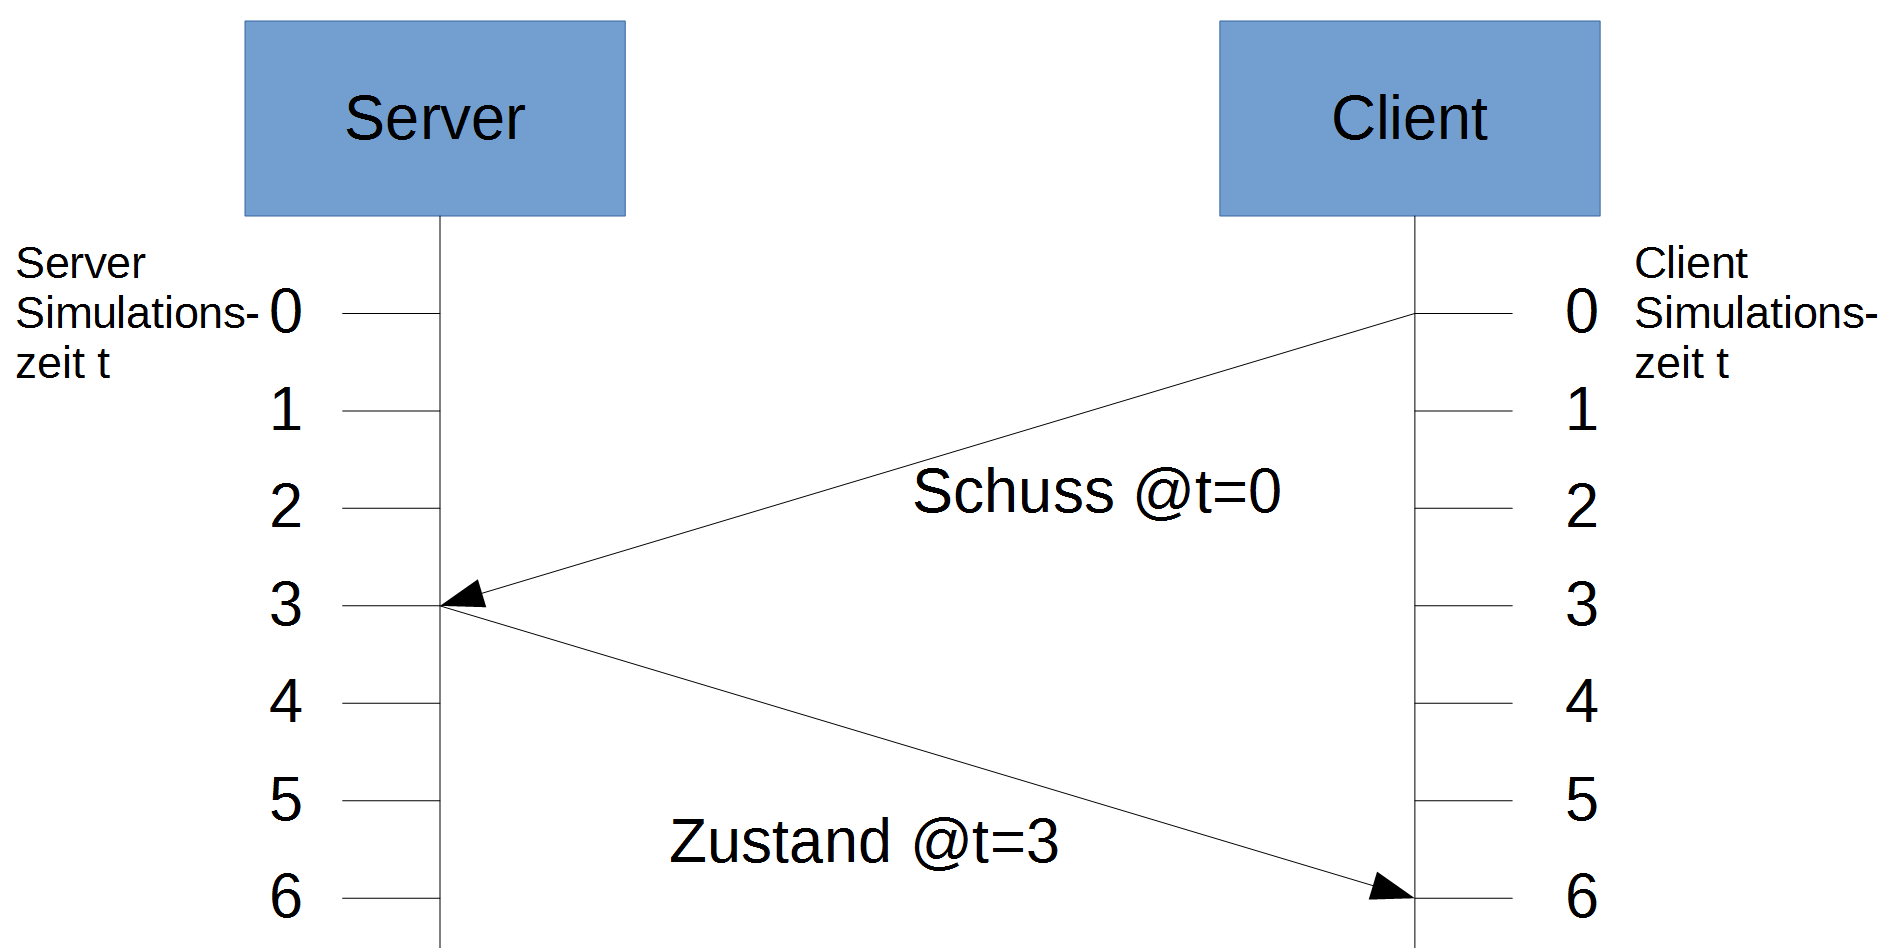
\includegraphics[width=0.75\textwidth]{./Zeichnung1a.png}
    \caption{Diagramm über Beispielsituation für Uhren, die gleichzeitig eingestellt sind. Gleiche Höhe entspricht Gleichzeitigkeit der echten Zeit. Dargestellt sind außerdem Beispielpakete mit Inhalt und Absendezeitpunkt in Simulationszeit.}
    \label{fig:zeichnung1a}
\end{figure}

Die offensichtlichste Variante der Einstellung der Simulationszeituhr am Client ist, möglichst Gleichzeitigkeit mit der Serveruhr anzustreben. Diese hätte allerdings Implikationen für die Implementierung, wie in Abb.~\ref{fig:zeichnung1a} ersichtlich. 
Aktionen, die vom Client ausgelöst werden, kommen erst verspätet am Server an.
Dieser müsste die so erhaltene Information retroaktiv anwenden, um die Richtigkeit aus der Sicht des Clients herzustellen.
Dann muss im schlimmsten Fall die gesamte Simulation wiederholt werden (von 0 bis~3), um einen korrekten Zustand zu Zeitpunkt~3 herzustellen. Dies benötigt Speicher, für die Speicherung alter Simulationszustände, und Rechenleistung zur wiederholten Neuberechnung von schon behandelten Simulationszeitpunkten. Den zweiten Teil der Arbeit hat der Client. Er erhält die Simulation zum Zeitpunkt~3 und muss daraus ein Bild für den Benutzer generieren, das den Zeitpunkt~6 darstellt. Dies kann auf 2 Arten erreicht werden.
\begin{enumerate}
\item Simulation am Client für die fehlenden Zeitschritte simulieren und das Ergebnis anzeigen. Dies hat den Vorteil, dass die Anzeige am Bildschirm am genauesten den echten Zustand darstellt, da alle Informationen in das Bild einfließen. Nachteile sind:
\begin{itemize}
 \item ein höherer Berechnungsaufwand, da die Simulation nun nicht nur am Server, sondern auch am Client stattfinden muss. 
 \item Der Server muss nicht nur Informationen, die die Anzeige am Bildschirm betreffen, versenden, sondern auch Werte, die nur für den Simulationsschritt wichtig sind.
 \item Wenn am Server etwas passiert, von dem der Client noch keine Informationen hat (z.B. Aktion eines anderen Spielers, die noch nicht angekommen ist), ist der Zustand der Simulation am Client nicht mehr valide. Der Client müsste dann also entweder alte Simulationszustände speichern und eine Neuberechnung durchführen, oder er ließe sich vom Server die komplette Simulation erneut zusenden.
\end{itemize}
\item Der Client rechnet die Anzeige auf unverbindliche Art und Weise nach vorne. Es wird hierbei dieselbe Extrapolation verwendet, die das Grafikmodul verwenden kann, um zwischen wenigen Simulationsschritten viele Bilder am Bildschirm zu erzeugen. Dazu werden vereinfachte Annahmen getroffen, wie z.B.~ dass Objekte sich linear bewegen, anhand der letzten bestätigten Position und letzten bestätigten Geschwindigkeit. Die resultierende Anzeigeposition wird nicht gespeichert, sondern nur zur momentanen Anzeige verwendet.
Vorteile sind die einfachere Berechnung und geringere benötigte Bandbreite vom Server. Außerdem hängt die benötigte Rechenzeit nicht davon ab, wie weit der letzte bestätigte Zeitpunkt zurückliegt. 
Nachteilig ist die geringere Genauigkeit der Anzeige gegenüber dem eigentlich korrekten Simulationszustand. Es werden auf dem Client so keine Interaktionen, wie z.B.~das Treffen eines Projektils, berücksichtigt. 
In der Praxis ist dies in den meisten Fällen aber nicht sehr kritisch, da innerhalb von Bruchteilen einer Sekunde der Server den Simulationszustand mit enthaltenen Auswirkungen von Interaktionen aktualisiert. Die grafische Diskrepanz zum Simulationszustand tritt also am Client nur für sehr kurze Zeit auf.\\
\end{enumerate}
\begin{figure}
    \centering
    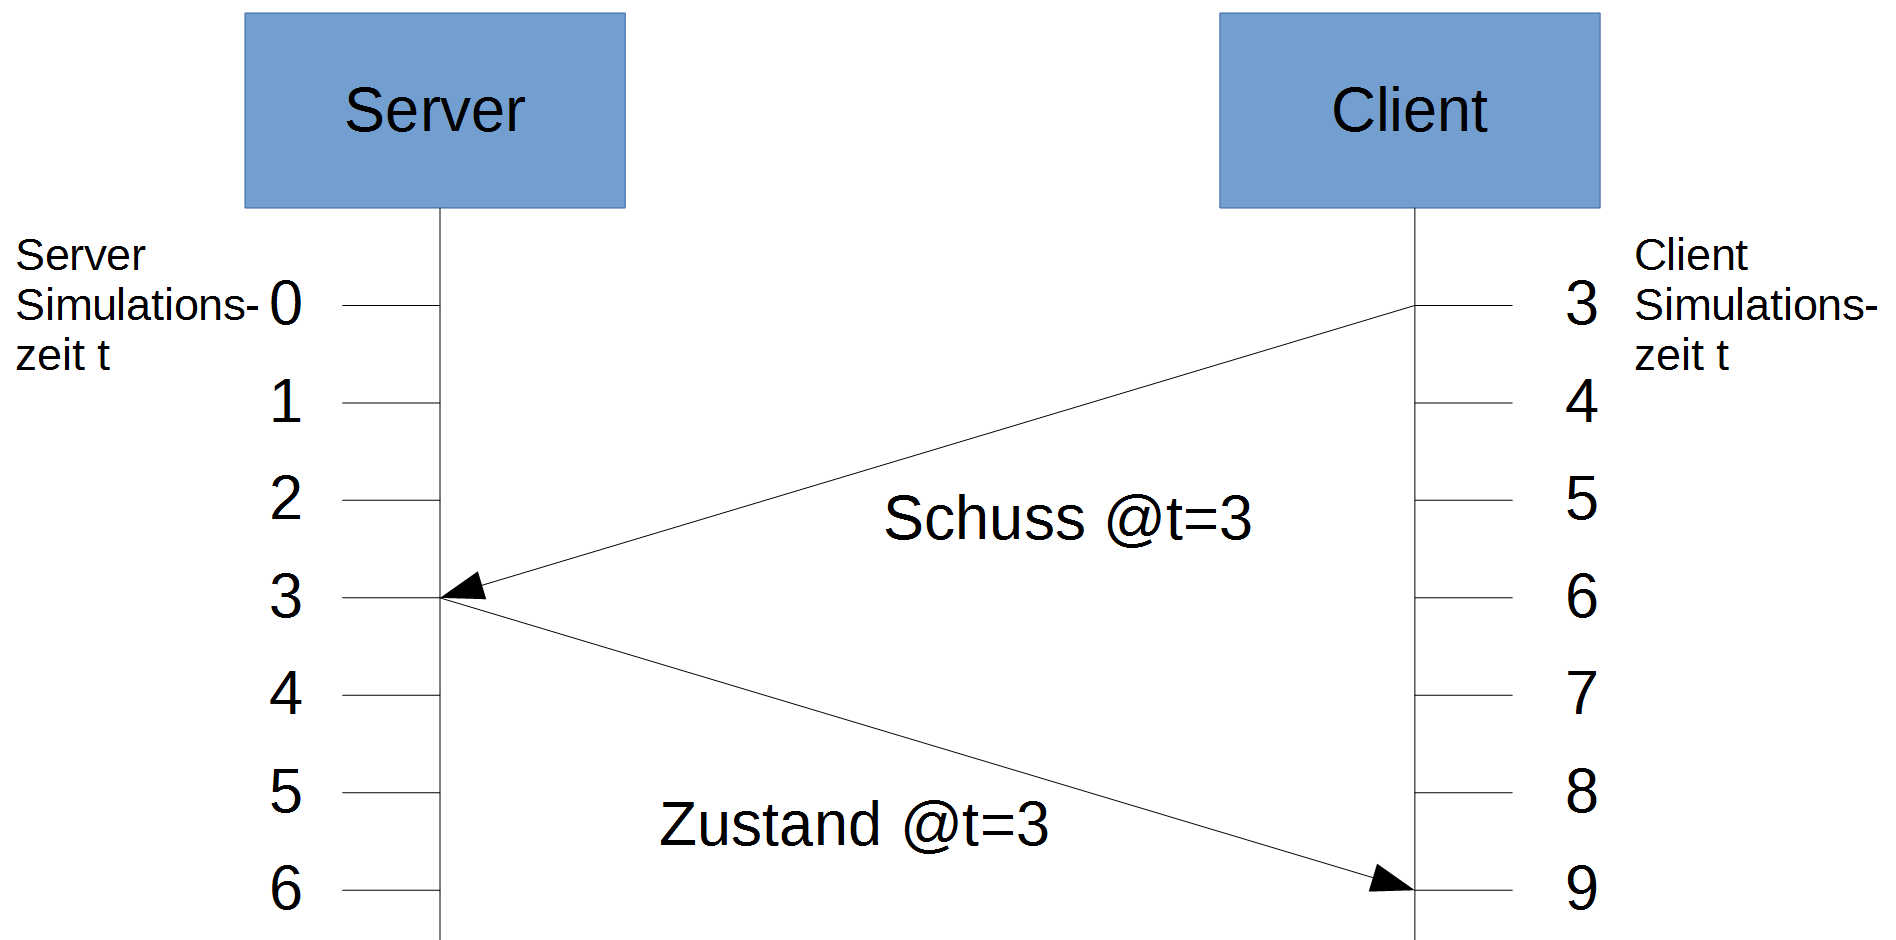
\includegraphics[width=0.75\textwidth]{./Zeichnung2a.png}
    \caption{Diagramm über Beispielsituation für Simulationszeit-Uhren, die zeitversetzt so eingestellt sind, dass der Client um die Latenz Client-zu-Server vorwärts zeitversetzt ist. Gleiche Höhe entspricht Gleichzeitigkeit der echten Zeit. Dargestellt sind außerdem Beispielpakete mit Inhalt und Absendezeitpunkt in Simulationszeit.}
    \label{fig:zeichnung2a}
\end{figure}
Eine weitere Möglichkeit, Uhren am Client einzustellen, ist die Uhr um die Einweg-Latenzzeit zum Server in die Zukunft zu stellen (siehe Abb.~\ref{fig:zeichnung2a}). In diesem Fall kann der Server die Aktionen vom Client als gegenwärtig betrachten und es müssen so keine retroaktiven Berechnungen durchgeführt werden.\\
Als Beispiel in der Abbildung dient der Schuss eines Projektils.
Der Schuss zum Zeitpunkt~3 des Clients ist also zu Zeitpunkt~3 am Server vorhanden, sodass er diesen wie eine lokale Eingabe in der Gegenwart verarbeiten kann. Speicherung alter Zustände oder wiederholtes Berechnen des selben Zeitpunktes sind nicht mehr nötig.
Aus diesen Gründen wurde dieses Modell gewählt. Der Server behandelt alle eingehenden Pakete mit Aktionen vom Client als in der Gegenwart auftretend.

Für den Client ändert sich gegenüber dem anderen Ansatz lediglich die Größe der Zeitdifferenz, die mit beiden o.g. Methoden zu einem aktuellen Bild führt. Für dieses Projekt wurde diejenige gewählt, die rein grafisch extrapoliert. Die grafische Diskrepanz zum Simulationszustand, obwohl nun u.U.~größer, wird immer noch als marginal eingeschätzt.\\

Die Berechnung von zeitverschobenen Ereignissen wird so nahezu komplett dem Client überlassen.
Das führt zudem zu einer hocherwünschten Robustheit des Simulationszustandes am Server gegenüber der Latenz, vor allem im Bezug auf hohe Latenzen zu einzelnen Clients. Die Simulation am Server ist auf diese Weise stabil, während die Seiteneffekte von hoher Latenz gerechterweise nur diejenigen Clienten betreffen, welche eine hohe Latenz zum Server haben.
Bei retroaktiven Strategien würden alle Clienten unter der hohen Latenz eines einzigen leiden, da dessen extrem verspätete Information so auf alle Clienten retroaktiv verteilt werden müsste.

%%TODO discussion : Mehrere spieler ? Latenztoleranz? Maximale vorausberechnung von Clients sonst drop? Ja, alles weitere Probleme aber wäre zuviel blah da das sowieso nicht das gewählte Modell ist.

\begin{figure}
    \centering
    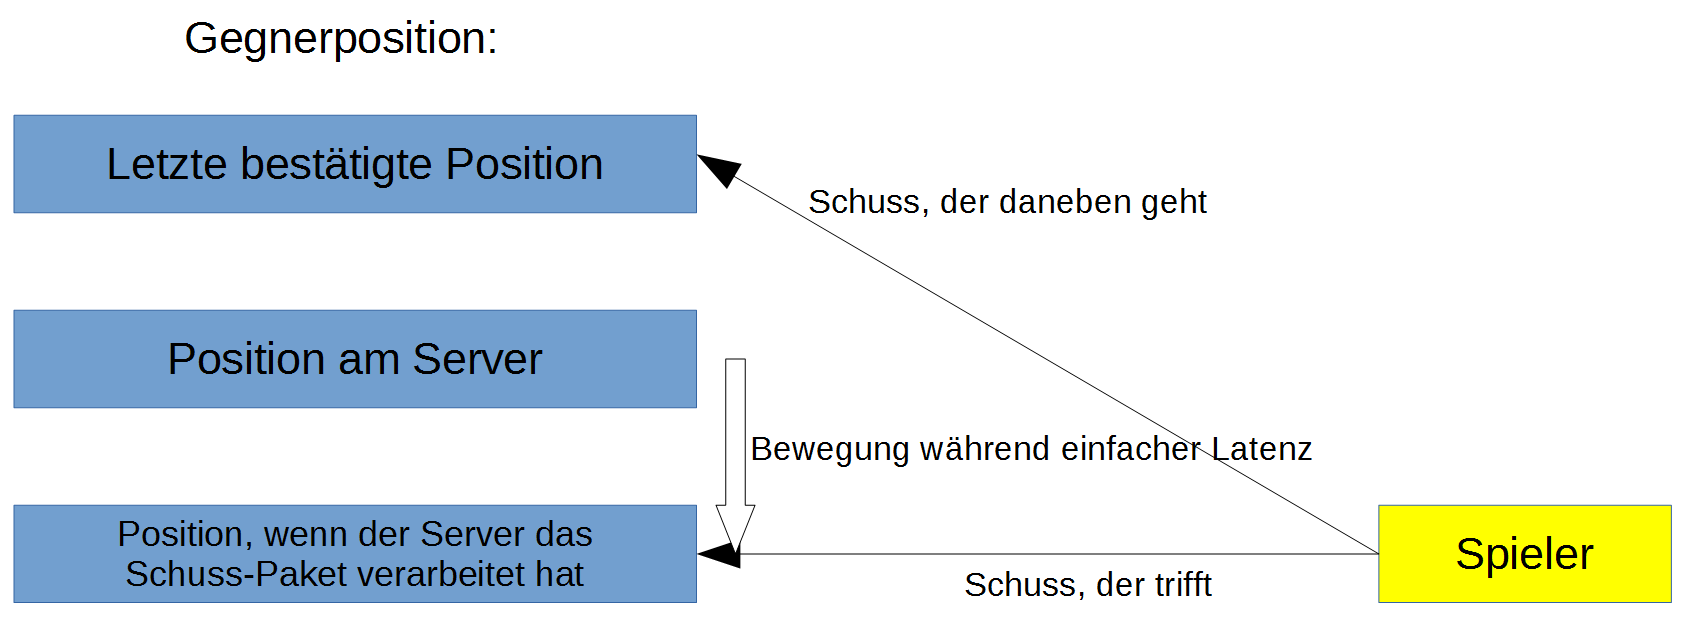
\includegraphics[width=0.85\textwidth]{./Gegnerposition1a.png}
    \caption{Diagramm über eine Beispielsituation, in der ein Spieler auf einen Gegner schießt. Der Ort im Diagramm entspricht größtenteils Maßstabsgetreu der Position in der Simulation (für Gegner, Spieler und Schüsse). Die einfachen Pfeile stellen Schüsse des Spielers dar.}
    \label{fig:gegnerposition1a}
\end{figure}

Der Grund dass die Extrapolation überhaupt notwendig ist, zeigt Abb.~\ref{fig:gegnerposition1a}. Die Berechnungslatenz und die Paketlatenz werden in der Implementierung (und in den Abbildungen) nur gemeinsam, als Gesamtlatenz verwendet. Zu sehen ist, dass wenn der Spieler auf die letzte bestätigte Position schießt, der Gegner sich zu einer neuen Position bewegt, bis die Informationen über den Schuss am Server ankommen. Der Schuss würde verfehlen. Die Aufgabe der grafischen Extrapolation ist es also, den Gegner an dem Ort anzuzeigen, wo er wahrscheinlich sein wird, wenn die Informationen über den aktuellen Client-Zustand in der Server-Simulation ankommen. Der Spieler kann dann wie lokal gewohnt auf bewegliche Ziele schießen, ohne die Latenz zum Server miteinbeziehen zu müssen.
Die Latenz, die für eine korrekte Extrapolation eingerechnet werden muss, muss die Zwei-Wege-Gesamtlatenz inklusive Berechnungslatenz auf Client und Server sein.\\

%%TODO TODO resolved?
Um die Daten für die oben beschribene Extrapolation möglichst genau zu ermitteln, bietet es sich an, die benötigten Daten an die normalerweise anfallende Kommunikation anzuhängen, die mit exakt der dafür korrekten Latenz arbeitet. Die Uhr des Servers wird als normales Datenelement (Syncable, später in Abschnitt~\ref{sec:syncable} beschrieben) an die Clients übertragen. Sie beinhaltet die aktuelle und gewünschte Simulationszeitrate relativ zur Realzeit (z.B. 0,1 bedeutet 10-fache Zeitlupe), und den aktuellen Zeitpunkt am Server. 
Client und Server versenden im Zuge der Latenzberechnung in jedem UDP-Packet ihre aktuellsten Realzeitstempel. Damit kann der Server den aktuellsten bekannten Zeitpunkt der Uhr für jeden Client mitführen. 
Dieser Zeitpunkt wird in jedem UDP-Packet, welches die Simulationsuhr auf dem Client aktualisiert, mitgeführt werden.
Wenn der Client nun ein Update der Uhr erhält kann er daraus die Zuordnung Realzeitzeitpunkt der Clientuhr zu Simulationszeitpunkt der Serveruhr (unter Berücksichtigung der Zeitrate) berechnen und so die Uhrensynchronisation beider Simulationszeituhren zwischen Client und Server herstellen. Ein Beispiel für das Verfahren ist in Abb.~\ref{fig:zeichnung3a} zu sehen.
\begin{figure}
    \centering
    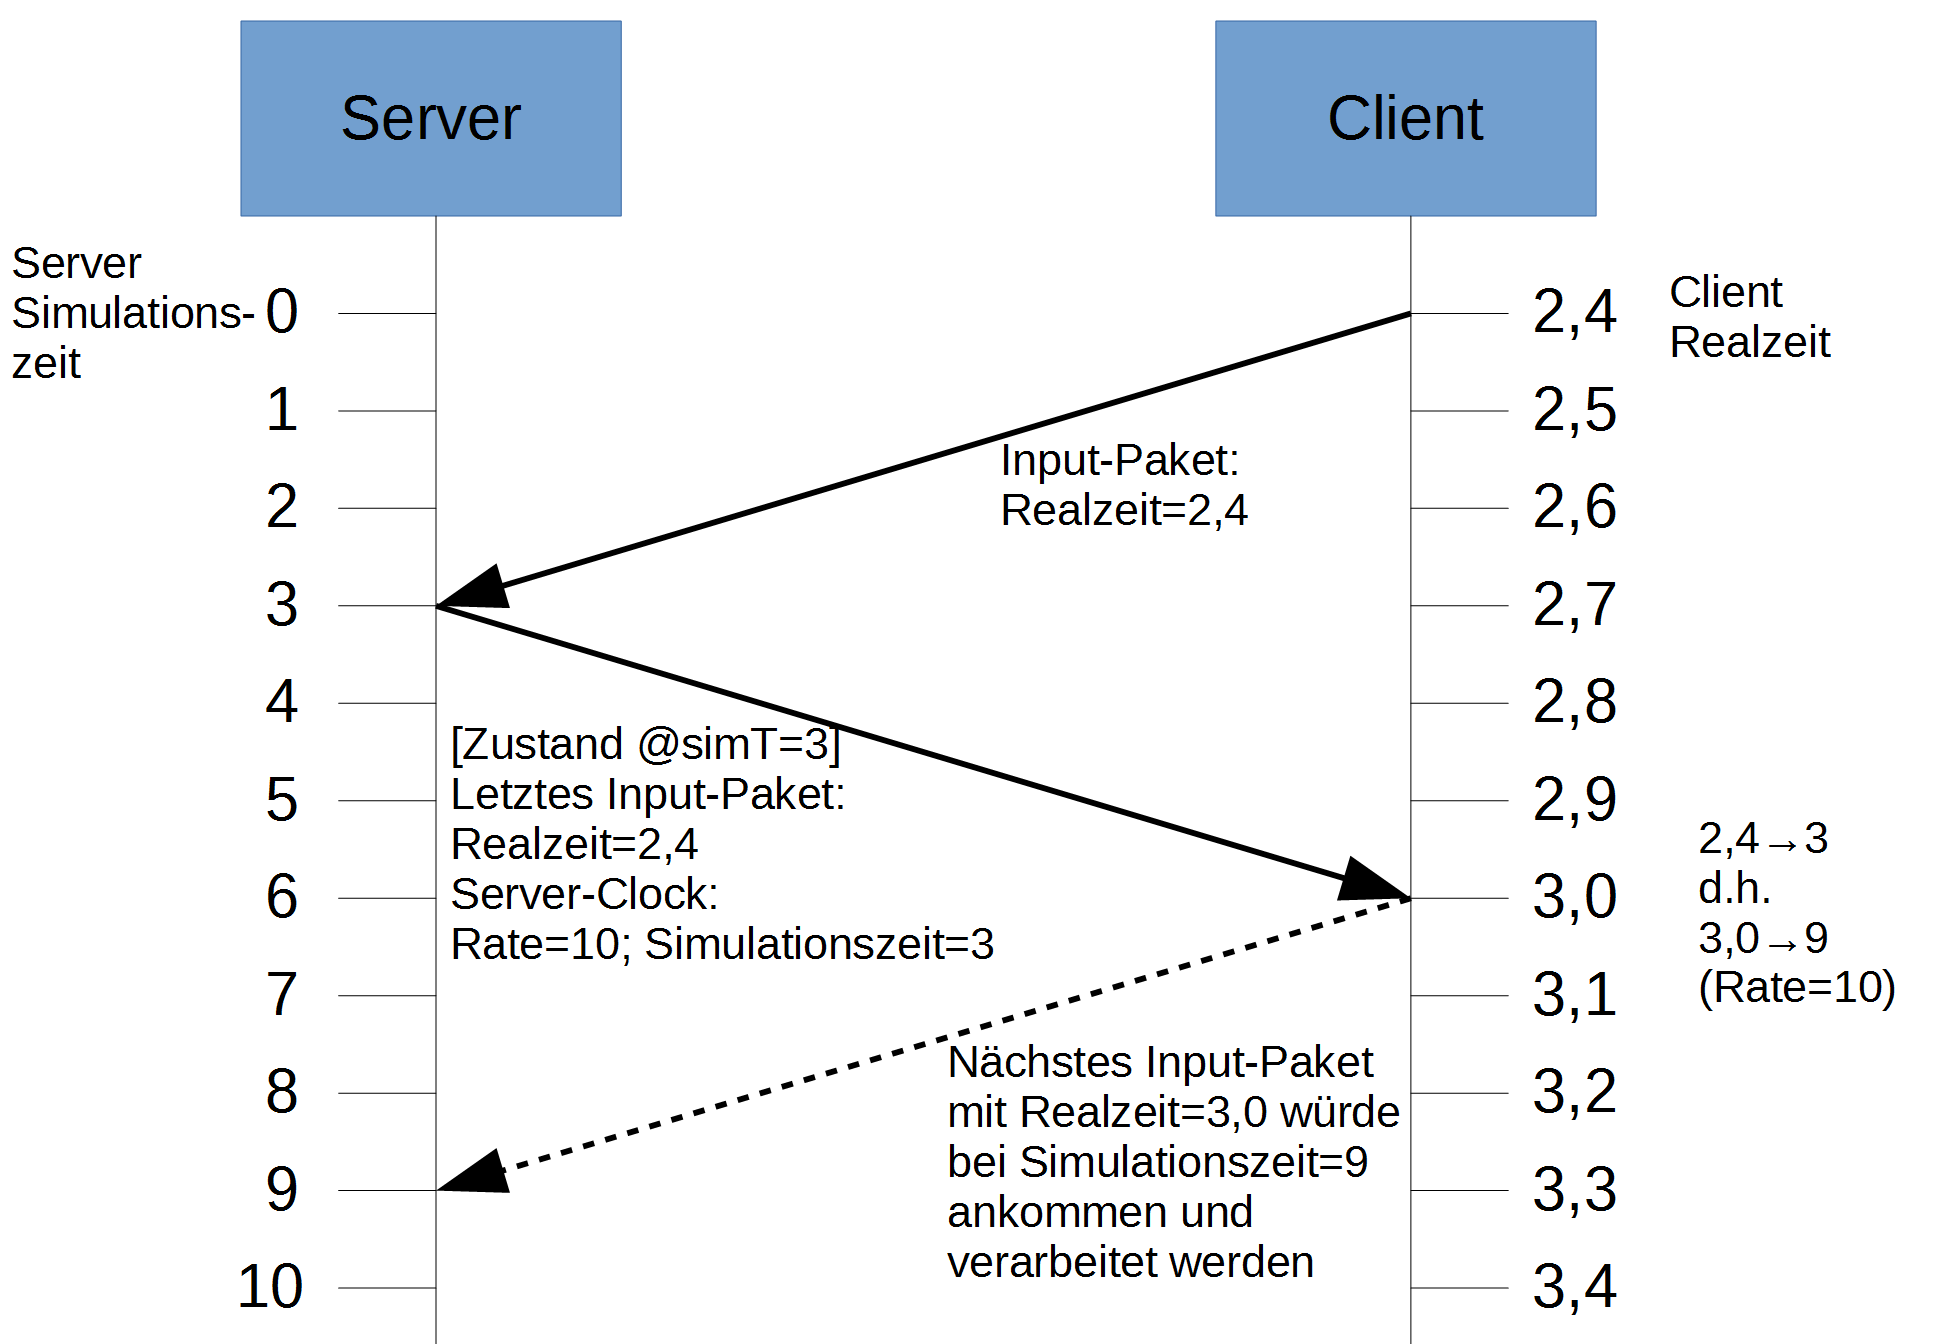
\includegraphics[width=0.75\textwidth]{./Zeichnung3a.png}
    \caption{Diagramm über Beispielsituation bei Simulationszeit-Uhrensynchronisation, mit zeitversetzten Uhren wie in Abb.~\ref{fig:zeichnung2a}. 
Gleiche Höhe entspricht Gleichzeitigkeit der physikalisch echten Zeit 
(nicht der Zeit, welche die jeweiligen Maschinen messen und als Realzeit interpretieren). Der Client errechnet aus den Daten in den Synchronisierungspaketen diejenige Simulationszeit, die dem Eintreffen am Server und der Verarbeitungszeit eines hypothetischen Pakets entspricht, wenn es sofort abgesendet werden würde.}
    \label{fig:zeichnung3a}
\end{figure}


\subsection{Übertragung der Simulationsinhalte zum Client}
\label{sec:syncable}
Um die Simulationsinhalte übertragen zu können, wurde zunächst ein Interface entworfen, über das die Daten gelesen und geschrieben werden können. Das Interface wird hier Syncable genannt.
Zunächst müssen die möglichen Datensätze in Kategorien unterteilt werden:
\begin{itemize}
\item Update-Daten: Daten, die ein bestehendes Objekt in den neuen, aktuellen Zustand überführen (z.B. Position)
\item Vollständiger Datensatz: Daten, die übertragen werden müssen, um ein neues Objekt zu erstellen. Diese Daten beinhalten meist alle Update-Daten und beinhalten zusätzlich noch die Daten, die einmalig zur Initialisierung notwendig sind (z.B. Größe eines konkreten Gegners).
\end{itemize}
Bei einem Syncable gibt es also eine Serialisierungs- und Deserialisierungsmethode. Um die gewünschte Kategorie auszuwählen, wird beim Aufruf zur Serialisierung ein Parameter übergeben, der dieser Auswahl entspricht. Die jeweilige konkrete Implementierung sammelt die jeweils relevanten Daten und hängt sie an das übergebene Paket an. Für das Paket wird die Programmbibliothek SFML, genauer deren Netzwerkkomponente, verwendet. Dadurch werden auch plattformspezifische Details wie z.B. Endianness automatisch berücksichtigt. Bei der Deserialisierung passiert der umgekehrte Prozess: Die Daten werden aus dem Paket entnommen und jedes Objekt führt das Update entsprechend durch. Bei der vollständigen Deserialisierung gibt es jedoch eine Besonderheit: Das Objekt existiert vor dem Aufruf noch nicht, weshalb statt einer Methode ein spezieller Konstruktor vom jeweils konkreten Objekt zur Verfügung gestellt wird, der aus den Daten des Pakets das Objekt initialisiert.
Dies weist auf ein weiteres Problem hin: Es muss zur Erstellung der konkrete Konstruktor aufgerufen werden, nicht nur eine abstrakte Methode. Dafür wird eine Factory verwendet. Damit der Typ eines Objekts übertragen werden kann, muss dieser anhand einer Klassen-ID mit einer abstrakten Methode abgefragt werden können. Die Factory auf der Gegenseite kann dann den konkreten Konstruktor für das Objekt aufrufen.
Im Rahmen des Projektes wurden also alle bestehenden Simulationsbestandteile, die übertragen werden müssen, zu Syncables. Für jedes davon wurden jeweils nur diejenigen Daten selektiert, die für die grafische Anzeige am Client relevant sind.

Syncables werden in einer Komponente, dem Syncable-Manager verwaltet. Wird der Server gestartet, wird die Simulation zur Initialisierung des Syncable-Managers verwendet. Die Simulation ist ebenfalls ein Syncable und agiert als Root, sodass Syncables in ihrem Besitz (alle Syncables der Simulation) in die Verwaltungsstruktur aufgenommen werden. Außerdem wird eine Benachrichtigungsstruktur eingerichtet, sodass bei Erzeugung von neuen Syncables in der Simulation der Syncable-Manager davon erfährt. Die Verwaltung erfolgt anhand IDs, die während der Aufnahme in die Struktur erzeugt werden und das Objekt über das Netzwerk identifiziert. Außerdem wird beim Einfügen ein Event erzeugt, das die ID, Klasse und alle anderen für die Initialisierung des Objekts notwendigen Daten umfasst (vollständige Serialisierung). Die Löschung eines Objekts wird ebenfalls über ein Event behandelt. Die Liste der Events (die schon als Binärdaten vorliegen) wird zyklisch von der Netzwerkkomponente gelesen und über TCP verschickt. An dieser Stelle überwiegen die Vorteile von TCP, da Events in der richtigen Reihenfolge und vollständig ankommen müssen.
Anders ist es bei Updates (Teilserialisierungen), die den Zustand eines bestehenden Syncables aktualisieren. Fehlende Updates sind unkritisch, da sie durch das nächste Update vollständig ersetzt werden. Veraltete Updates, die verspätet ankommen können einfach verworfen werden. Aus diesen Gründen ist hier UDP die beste Wahl.
Bei Events ist die benutzte Bandbreite durch die Anzahl und Größe der Events festgelegt, da sie nicht weggelassen werden können. Bei Updates bedeutet ein fehlendes Paket jedoch nur eine etwas ungenauere Positionsextrapolation, die die Grafikkomponente erzeugt. Die Rate, mit der Updates versendet werden, kann also variabel gewählt werden. Da Netzwerkverbindungen immer eine Bandbreitenlimitierung aufweisen, sollte diese beachtet werden und als Grenze für die Rate der Updates dienen. Die Netzwerkkomponente verwaltet die maximale Bandbreite, indem die TCP-Bandbreite gemessen wird und der Rest einer einstellbaren Maximalbandbreite für Updates zur Verfügung steht. In den zyklischen Anfragen an den Syncable-Manager fordert die Netzwerkkomponente Pakete mit maximaler Größe an. Darin werden solange Updates von einzelnen Syncables eingefügt, bis das die Maximalgröße ein weiteres Einfügen verhindert. Die Syncables, die im aktuellen Paket enthalten sind, werden nach dem Round-Robin-Verfahren ausgewählt (maximal 1~Runde pro Zyklus). Die Zustellung der Updates am Client erfolgt anhand der ID der Syncables.


\subsection{Besonderheiten}
Die Implementierung weist noch einige Besonderheiten auf:
\begin{itemize}
\item Das Terrain wird nicht übertragen, da es mit einem plattformunabhängigen Zufallsgenerator mit festem Seed erzeugt wird und daher auf den verschiedenen Rechnern identische Resultate liefert. Terrain kann sich außerdem nicht verändern. Aus diesen Gründen kann der Client es einfach selbst bei Bedarf erzeugen (und wieder verwerfen, sobald sich der Spieler von einem Ort zu weit entfernt).
\item Die Sichtrichtung des Spielers wird aktuell noch vom Server bestimmt, ohne dass der Client für die Kamera im 3D-Raum eine eigene Schätzung benutzt. Dies bedeutet, dass der Spieler die Kamera nur über den Umweg zum Server drehen kann und dabei eine Latenz in Kauf nehmen muss. Die Latenz der Kameradrehung ist jedoch bei First-Person-Shootern diejenige, die den größten negativen Einfluss auf sowohl Spielspass als auch Spielerleistung hat. Dies wäre somit die höchste Priorität für Erweiterungen des klassischen linearen Extrapolationsmodells der Grafik am Client. Problematisch bei der Umsezung ist dort der Fakt, dass der Server bestimmt, wann der Spieler seine Waffe abfeuert. Er bestimmt damit auch den Rückstoß, der die Blickrichtung ändert.
\item Das Löschen von Syncables (auf Befehl des Servers) kann nicht abstrakt erfolgen, da verschiedene Klassen von verschiedenen Komponenten verwaltet werden und die jeweils korrekte über die Löschanfrage benachrichtigt werden muss. Über die in Abschnitt~\ref{sec:syncable} beschribene Klassen-ID ist eine Differenzierung zur Laufzeit möglich.
\item Sounds, die alle als Reaktion auf ein Ereignis im Spiel auftreten (also vom Server angeordnet werden), wurden im Rahmen des Projekts nicht synchronisiert. Der Grund dafür ist, das aufgrund der Art und Weise, wie sie bisher implementiert sind, eine weitgehende Neuimplementierung des Features notwendig wäre, um auf dem Client zu funktionieren. Dies wäre für den Rahmen des Projekts zu viel Aufwand. 
\end{itemize}





\section{Zusammenfassung}
Da die Arbeit an der Codebasis nicht auf das HSP-Projekt beschränkt ist, ist eine zukünftige Arbeit an einer Verbesserung der Synchronisation wahrscheinlich. Der aktuelle Stand weist noch einige Probleme und einiges an Optimierungspotenzial auf:
\begin{itemize}
\item Die Sichtrichtung einer Spielerfigur, und somit die grafisch angezeigte Perspektive am Client, wird aktuell noch vom Server bestimmt, ohne dass der Client für die Kamera im 3D-Raum eine eigene Schätzung verwendet. 
Ein Spieler muss so beim Drehen seiner Sicht die Zwei-Wege-Latenz zum Server in Kauf nehmen. Zwar handelt der Server nach dem hier gezeigten Synchronisationsschema mit Gleichzeitigkeit, der Unterschied wird jedoch am Client grafisch merkbar, wenn sich die Perspektive schnell ändert während z.B.~geschossen wird. Projektile sind prinzipiell da wo sie sein sollen, das lokal angezeigte Fadenkreuz u.U.~allerdings nicht. Für einen Shooter ist die Flüssigkeit des Bildes  beim Zielen essentiell.
Dies wäre somit die höchste Priorität für Erweiterungen des klassischen linearen Extrapolationsmodells der Grafik am Client, die lokal anliegenden Eingabeereignisse eigenständig mit einzubeziehen. Problematisch bei der Umsezung ist dort, dass der Server bestimmt, wann der Spieler seine Waffe abfeuert. Er bestimmt damit auch den Rückstoß, der die Blickrichtung ändert.
\item Geräusche, die alle als Reaktion auf ein Ereignis im Spiel auftreten (also vom Server angeordnet werden), wurden im Rahmen des Projekts nicht synchronisiert. Der Grund dafür ist, das aufgrund der Art und Weise, wie diese bisher implementiert sind und eine weitgehende Neuimplementierung des Features notwendig wäre, um auf dem Client zu funktionieren. Das wurde für den Rahmen des Projekts als zu Aufwändig eingeschätzt.
\item Informationen sind aktuell nicht priorisiert. Es wäre jedoch für die gefühlte Latenz von Vorteil, wenn Updates z.B.~zur eigenen Spielfigur in jedem Paket enthalten wären, und nicht nur, wenn diese im Round-Robin Verfahren an der Reihe is. Da aber aktuell der Syncable-Manager nur ein einziges Paket erzeugt, das von der Netzwerkkomponente an alle Clients gesendet wird, muss dort eine signifikante Anpassung erfolgen, um für unterschiedliche Clients unterschiedliche Updates zusammenzustellen. Über ein ähnliches System könnte man außerdem die Genauigkeit von Update-Paketen auf den konkreten Client zuschneiden. So wäre es z.B. vertretbar, bei einem weit entfernten Gegner dessen Sichtrichtung nur mit einer Genauigkeit von 1\,Byte pro Achse zu übertragen.
\item Die bisherige Implementierung erlaubt neben einzelnen Kreierungen und Löschungen von Objekten auch die Einbindung beliebiger Events. Über diese könnte man bisherige bandbreitenintensive Kreierungsbefehle zu Gruppen zusammenfassen, die z.B. mit einem deterministischen Pseudozufallsgenerator auf beiden Maschinen mit minimalem Datenaustausch identische Resultate liefern. Man könnte diese Events außerdem benutzen, um die Updates für eine große Menge an Entitäten zu ersetzen. Dies wäre möglich, indem diese in einer Gruppe zusammengefasst wären und intern deterministisch agieren (z.B Gegner marschieren in Formation). Die übertragenen Events wären dann Befehle, die deterministisch die Aktionen über einen bestimmten Zeitraum bestimmen.
\item Der Client könnte komplexere Vorausberechnungen als die lineare Extrapolation anstellen. So könnte er z.B. temporäre Entitäten erzeugen, die nur solange existieren, bis Serverinformationen über deren Erstellungszeitpunkt den Client erreicht haben. Sie würden dann durch die aktuellen Informationen vom Server ersetzt werden (oder ersatzlos gestrichen, wenn der Server für diesem Zeitpunkt keine Erzeugung einer Entität vorgesehen hat). So könnte der Spieler z.B. lokal ein abgeschossenes Projektil sofort sehen, nicht erst wenn es vom Server bestätigt wurde.
\end{itemize}

\newpage

\printbibliography
\newpage

\appendix
\section{Beschreibung und Spezifikation von Kernkonzepten einer 3D-Simulation mit dem Fokus auf die Verwendung als Videospielplattform}
\label{appendixA}
\subsection{Einleitung}

Die folgenden Abschnitte dienen als Beschreibung und Spezifikation für ein 3D-Simulationsprogramm, welches für die Umsetzung diverser Videospielideen konzipiert ist.
Es sollen ausgewählte Aspekte der Simulation deklarativ beschrieben und/oder möglichst unmissverständlich spezifiziert werden, ohne eine konkrete Umsetzung zu sehr einzuschränken.
Das Dokument kann ebenfalls detaillierte Informationen zur derzeitigen Umsetzung bestimmter Aspekte der Simulation liefern.

Einige Begriffe im Kontext von Videospielen sind in der wissenschaftlichen Literatur nur wenig vertreten, jedoch in der Szene fest etabliert. Diese sollen hier ebenfalls eindeutig definiert werden, um ggf.~ defizite verfügbarer Quellen auszugleichen.

\subsection{Problemdefinition}
Die Erstellung einer 3D-Simulation umfasst die Kreation eines beschränkten Universums. Diese grandiose aber treffende Erkenntnis hilft, die grundlegenden Konzepte der Simulation zu identifizieren. Im folgenden sollen solche, aber auch technologische Konzepte für die Simulation spezifiziert werden.\\
Da mathematische Notation nicht standardisiert ist, wird sich dabei an definierte mathematische Konzepte der mathematischen Z-Spezifikationssprache angelehnt. Bei Unklarheit bezüglich der mathematischen Syntax in diesem Dokument kann die Quelle \cite{Z} zu Rate gezogen werden. 

Die 3D-Simulation umfasst hier die Echtzeitsimulation von Entitäten in einem 3D-Kontext. Darin enthalten sind ebenfalls die Aufgaben der Video- und Audioanzeige des Inhalts der Simulation und die Steuerung von bestimmten Inhalten in Echtzeit.\\
Die konkreten Ausmaße des Problems der Erstellung dieser Simulation ist von den Features der zu simulierenden Entitäten abhängig.

Um einen grundlegenden Einblick zu bieten können einige der umgesetzten, bzw. angestrebten Features für diese Simulation beispielhaft beschrieben werden.\\
Klassischerweise im Kontext der 3D-Simulation per se umfasst dies:
\begin{enumerate}
\item Rigide physikalische Objekte
\item passiv physikalische rigide Objektkollision
\end{enumerate}

Im Kontext eines Videospiels können weitere Aspekte hinzugefügt werden. Einige sind dabei abhängig vom jeweiligen zu realisierenden Videospiel:
\begin{enumerate}
\item Projektile
\item Nicht Spieler Charactere (NPC)/Gegner
\item Spieleravatare\\
Von einem Benutzer Steuerbare Entitäten, welche diverse Aktionen ausführen können.
\item Terrain
\item diverse benutzbare Gegenstände/Items und Inventare (Werkzeuge/Waffen)
\end{enumerate}






\subsection{Datentypen}
Durch physikalische und technologische Begrenzungen schränkt eine Rechenmaschine mathematischen Zahlenräume ein:
\begin{itemize}
\item Für die Darstellung von Reelen Zahlen $\mathbb{R}$ werden meist Floating-Point-Datentypen verwendet. Wir verwenden hier hauptsächlich 32-Bit IEEE Floats mit einfacher Genauigkeit. Die Verwendung von doppelter Präzision in der Zukunft soll nicht ausgeschlossen werden.
Die Menge an so repräsentierbaren Zahlen soll hier im weiteren mit $\mathcal{F} \subset \mathbb{R}$ bezeichnet werden.
\item Integer $\mathbb{Z}$ sind hier durch maximal 64-Bit beschränkt. Diese beschränkte Menge an Integern wird $\mathcal{I} \subset \mathbb{Z}$ genannt. Die exakte Größe des Integers kann jedoch je nach Verwendungszweck variieren.
\end{itemize}


\subsection{Zeit}
\label{sec:time}
\def\finite#1{\ooalign{\hfil$\mapstochar\mkern 3mu\mapstochar\mkern 5mu$\hfil\cr$#1$}}

Die Simulation läuft gezeitet ab.
Es existiert auf einer Rechenmaschine eine Uhr, deren zeitliche Referenz verwendet wird.
Auf Basis der Uhr definieren wir zwei relevante zeitliche Sequenzen:
\begin{enumerate}
\item Die maschinell abgetastete, diskrete Realzeit der echten Welt $T_r:=\langle t_{epoch}, ... , t_{max}\rangle$

\begin{itemize}
	\item $t_{epoch}, t_{max}$ als minimal, bzw.~maximal darstellbare Zeit
	\item In einer maschinellen Genauigkeit in Mikrosekunden 
\begin{align}
	\epsilon_t:=10^{-6}s ; \forall c \in \mathbb{Z}: T_r(c) + \epsilon_t = T_r(c+1)
\end{align}
	\item und immer streng monoton wächst 
\begin{align}
	\forall c \in \mathbb{Z}: T_r(c) < T_r(c+1)
\end{align}
	\end{itemize}

\item Die Simulationszeit $T_s := \langle t_{start}, ... , t_{end}\rangle$
	\begin{itemize}
	\item $t_{start}, t_{end}$ als Start- und Endzeitpunkt der Simulation.
	\item Zwischen den beiden Zeitbasen besteht eine totale, nicht-injektive, surjektive Abbildung. Die Simulationszeit ist dadurch relativ zur Realzeit definiert.
\begin{align}
	\mathcal{T}:T_r \twoheadrightarrow T_s
\end{align}
	\item Um die Kontinuität der Zeit herzustellen wird weiter eine flexible Zeitrate $r_t$ in Abhängigkeit zur Realzeit definiert, welche das relative Verstreichen der Zeit in der Simulation steuert. 
\begin{align}
r_t:T_r\mapsto\mathcal{F}\\
 \forall t_{r0},  t_{r1} \in T_r ; t_{diff}=t_{r1}-t_{r0} :\mathcal{T}(t_{r1}) = \mathcal{T}(t_{r0}) + t_{diff}\cdot r_t(t_{r1})
\end{align}
Die Rate bleibt während aller Zeiten zwischen $t_{r0}$ und $t_{r1}$ gleich.
\begin{align}
 \forall t \in [ t_{r0},t_{r1}]: r_t( t_{r0}) = r_t(t)
\end{align} Wird die Eigenschaft des Zeitflusses in der festgelegten Rate verletzt, werden die aktuellen Echtzeitanforderungen verletzt. \\
	Soll die Rate also geändert werden muss dies zu festgelegten Umschaltpunkten geschehen, welche die Simulationszeit in Zeitbereiche trennen, zwischen denen keine Berechnungsvorgänge zuverlässig durchführbar sind.\\
Beispiele für Raten sind 
\begin{itemize}
\item $r_t(x) = 1 \Leftrightarrow$ Simulation synchron zur Echtzeit
\item $r_t(x) = 0 \Leftrightarrow$ Simulation ist pausiert/läuft nicht
\end{itemize}
Technisch wird für große $|r_t|$ die Simulation schwierig, da viele Vorgänge schnell simuliert werden müssten. Diese werden daher vermieden.\\
Theoretisch kann die Rate auch negative Werte annehmen. Die Simulationszeit würde dann rückwärts laufen. Dieses Verhalten ist technisch durch die monoton steigende Realzeit nicht leicht in konsistenter Weise umzusetzen, da Realzeiteinflüsse durch Tasteneingaben existieren und soll daher hier ebenfalls vermieden werden.
	\end{itemize}
\end{enumerate}	

\subsection{Tick \& Frame}
\label{sec:tick}
Die Simulation behandelt das Verstreichen von Zeit in Zeitschritten, während dem der interne Zustand der Simulation, bzw.~der simulierten Objekte, zu einem zeitlich neuen Zustand aktualisiert wird.
Dieser Zeitschritt, bzw.~Verarbeitungsschritt, wird als Tick bezeichnet \cite{tick}.
Es ist besonders anzumerken, das der Begriff des Ticks sich ausschließlich auf das Voranschreiten der Simulation auch bei kompletter Abwesenheit einer graphischen Renderingpipeline bezieht. Im grafischen Kontext wird dafür der Begriff Frame (dt. Bild) verwendet, da der äquivalente Prozess der Grafik einmal pro Rendern und Anzeigen eines Bildes geschieht.\\

Von beiden Größen können Raten $r_{tick}, r_{frame} \in \mathbb{R}$ angegeben werden (üblicherweise in Tick/Frame pro Realzeitsekunde). Praktisch kann eine Grafikengine durch Inter- oder Extrapolation dynamisch verschiedene, von der Tickrate unabhängige Frameraten erreichen.\\

Bei einer unsauberen Trennung der beiden Rate treten Inkonsistenzen in der Simulation in Abhängigkeit der Framerate auf (Beispiel: In \glqq The Elder Scrolls V: Skyrim\grqq lernen Mammuts auf Grund falscher physikalischer Berechnungen in Abhängigkeit von zu hohen Frameraten das Fliegen \cite{flying-fucking-mammoths}).

Es existiert dort dann meist eine maximale Framerate.
Dieser Umstand scheint die Problematik mitzuführen, dass viele Videospielhersteller, vor allem im Konsolenbereich, Frameraten immer weiter nach unten limitieren, um ihre Produkte umzusetzen, was die Qualität erheblich senkt (Beispiele \cites{skyrim-physics-cap-and-fix, dark_souls-physics-cap-and-fix})
(entgegen der Meinung ihrer Marketingabteilungen, mit einer Menge negativer Presse, Beispiele \cites{morecinematic00, morecinematic01}
) und dazu führt dass Benutzer ihre u.U.~teure, fähige Hardware nicht ausnutzen können und sich mit schlechter Bildqualität zufrieden geben müssen.\\
Ein Umstand, der oft auf umständlichem Weg durch fähige Konsumenten selbstständig gelöst wird (vgl. \cites{skyrim-physics-cap-and-fix, dark_souls-physics-cap-and-fix})
Die Trennung von Physik und Grafik scheint eine grundsätzliche Designentscheidung zu sein, die in vielen kommerziell genutzten Engines fehlt.

Wir definieren einen Tick anhand seiner realen, ersten Auftrittszeit
\begin{align}
\delta_t: t \in T_r
\end{align}
Wir notieren in einem Tick enthaltene Realzeitpunkte als
\begin{align}\label{m:tickinterval}
\delta_{t_d}; d \in [0,1]
\end{align}
und bezeichnen daher Tickbeginn, bzw.~-ende als $\delta_{t_0}$, bzw.~$\delta_{t_1}$. 

Die Inklusivität/Exklusivität der Intervallgrenzen eines Ticks (\ref{m:tickinterval}) muss in bestimmten Berechnungskontexten manchmal angepasst werden um bei sukzessiven Ticks doppelte Behandlungen von Ereignissen zu vermeiden. Diese Einschätzung sei für jeden Kontext individuell zu vollziehen.
Es gilt außerdem die Kontinuität der Zeit auch bei Ticks , d.h. ein Tick beginnt am Endzeitpunkt des Vorherigen.
\begin{align}
	\delta_{j_1} = \delta_{(j+1)_0}\label{m:tick_continuity}
\end{align}
Dadurch kann eine realzeitlich geordnete Sequenz von Ticks angegeben werden
\begin{align}
	\delta := \langle \delta_t, ... \rangle ; t \in T_r
\end{align}
Da die Sequenz eine klare Ordnung der Ticks angibt ist auch eine Indexschreibweise möglich, um einen Tick zu spezifizieren.
\begin{align}
	\delta_i := \delta(i); i \in \mathbb{N}
\end{align}
Durch die Abbildung $\mathcal{T}$ erhält der Tick eine Entsprechung in Simulationszeit.\\
Ist im aktuellen Kontext nur ein Tick $\delta_i$ von Belang, wird auch die Terminologie 
\begin{align}
t_d = \mathcal{T}(\delta_{i_d})
\end{align}
, also $t_0$ für den Tickbeginn und $t_1$ für dessen Ende in Simulationszeit, verwendet.\\
Man kann weiter eine Sequenz als die zusammenhängende Partition der Simulationszeitsequenz $T_s$ denotieren, welche die geordneten Zeitpunkte eines Ticks in Simulationszeit enthält.
\begin{align}
\Upsilon_{\delta i} = \langle t_0, ...,  t_1\rangle
\end{align}
Die in Abschnitt~\ref{sec:time} beschriebenen möglichen Umschaltzeiten zur Änderung der Zeitflussrate in der Simulation werden auf die Grenzen von Ticks gelegt.\\
Die Größe der Zeitdifferenz $t_1 - t_0$ unterliegt meist Einschränkungen. Bestimmte Simulationsalgorithmen wie z.B. die Methode der kleinen Schritte erfordern für eine bestimmte Genauigkeit eine maximale Schrittgröße. Die verfügbare Rechenleistung hingegen beschränkt die Tickrate nach oben. Reicht die Berechnungszeit während eine Ticks nicht um den Status der Simulation von $t_0$ auf $t_1$ zu aktualisieren, läuft die Simulation langsamer als die reale Zeit. Die Echtzeitanforderung ist dann verletzt. Oft wird die Tickrate als Konstante festgelegt, in diesem Projekt ist jedoch nur eine Mindestrate festgelegt.\\
Das Konzept eines Ticks und dessen Mindestrate war schon vor dem Projekt in der Codebasis enthalten, die Implementierung erfuhr jedoch einige Anpassungen.

\subsection{Raum}
\label{sec:space}
Ein Raum wird durch eine Punktemenge definiert, welche alle darstellbaren Punkte eines Koordinatensystems umfasst. Hier werden meist kartesische Koordinatensysteme verwendet.\\
Die Größe und Granularität des Raums wird dabei durch verwendete Längendatentypen in dreidimensionalen Vektoren bestimmt.\\
Ein Kandidat für einen solchen Längendatentypen ist ein Floating-Point-Datentyp  $\mathcal{F}$, der den Raum in der Einheit Meter beschreibt.\\
Durch die Werteverteilung in $\mathcal{F}$ treten jedoch für Positionen mit absoluter großer Entfernung zum Ursprung $O$ Genauigkeitsverluste auf, die zur Verletzung von Genauigkeitsanforderung führen können. 
Die Ursache: Floating-Point-Werte liegen dichter beieinander, je näher am Ursprung \cite{floatdistribution}. Ein Beispiel für die möglichen Auswirkungen dieses Sachverhalts in Simulationen kann in der Quelle \cite{floatdistributionexample} betrachtet werden.\\
Physikalische Prozesse berechnet auf Basis von Positionen in $\mathcal{F}^3$ können daher inkonsistent in Abhängigkeit zum Ort im Raum sein.\\
Das Problem wird hier durch einen neuen Längendatentypen 
\begin{align}
	\mathcal{S} : \mathcal{I} \times \mathcal{F}
\end{align} gelöst, welcher den Raum zunächst gleichmäßig durch $\mathcal{I}$ aufteilt und indiziert und $\mathcal{F}$ als Offset innerhalb seines Raumteils verwendet. 

Es wird daher eine Größe der initialen Aufteilung $\gridsize$ in Metern definiert.\\
Die Umrechnung Typs $\mathcal{S}$ zur Darstellung in $\mathcal{F}$ in Metern ist dann:

\begin{align}
	f \in [0;1[ \label{m:S_unique} \\
	\tometer: \mathcal{S} \mapsto \mathcal{F};  \tometer((i, f)) = i \cdot \gridsize + f \cdot \gridsize
\end{align}
Die Bedingung \ref{m:S_unique} realisiert die Eindeutigkeit von Repräsentationen für Punkte.

Diese Darstellung hat folgende weitere Vorteile
\begin{itemize}
\item Einfache Implementierung
\item Schnelle Indizierung der durch $\mathcal{I}$ indizierten Raumanteile für raumaufteilende Algorithmen
\end{itemize}

Absolute Positionen im Raum werden demnach mit Vektoren $\mathcal{S}^3$ dargestellt. Für Berechnungen von Interaktionen zwischen Objekten werden Positionen zunächst zueinander relativiert und nach $\mathcal{F}^3$ umgewandelt, um so hardwaregestütz Berechnungen durchzuführen. 
Man geht dabei davon aus, dass relative Strecken zwischen Objekten kurz genug sind, sodass die Genauigkeitsänderung in $\mathcal{F}$ vernachlässigbar ist.\\
Effektiv ist dabei die Eigenschaft $\mathcal{F}\subset\mathcal{S}$ nicht exakt gefordert, auch wenn sie in der in diesem Projekt verwendeten Implementierung prinzipiell gilt.

Im Rahmen der Simulation bestehen diverse kartesische Koordinatensysteme, bzw. Räume. Entitäten werden je nach Anwendungsfall zweckmäßig zwischen diesen Transformiert, um bestimmte Features abzubilden.

\begin{enumerate}
\item Weltraum (Worldspace)in $\mathcal{S}^3$; absolute Positionen
\item Kameraraum (Cameraspace) in $\mathcal{F}^3$; Ursprung $O$ ist die Position der Kamera zum Rendern einer Szene, Objekte werden zur Kamera relativiert.
\item Sichraum (Viewspace) in $\mathcal{F}^3$; Verzerrung durch die Kameralinse, um einen Blickwinkel auf einen Bildschirm anzupassen.
\item Objektraum (Objectspace) in$\mathcal{F}^3$; Ursprung ist der vom Modell definierten Mittelpunkt eines Objektes (Massenmittelpunkt). Jede Objektform kann in seinem eigenen Objektraum definiert werden. Zur Verarbeitung von physikalischen Objektinteraktionen wird ein Objekt zu einem anderen Objekt durch Transformation in dessen Objektraum relativiert.
\end{enumerate}

Auf diese Weise gelingt es selbst extreme absolute Entfernungen und Geschwindigkeiten im Relativen akkurat zu behandeln.

\subsection{Entitäten}
\label{sec:entity}

Entitäten sind der atomare Inhalt der Simulation. Es handelt sich dabei um eine Abstraktion für \glqq Etwas\grqq ~in der Simulation. In der Realität suchen Physiker immer weiter \glqq Das [sie] erkenne[n], was die Welt im Innersten zusammenhält, ..\grqq [J.W.v. Goethe, Faust, \glqq Nacht\grqq, Vers. 382]. Was in der Realität eine offene Frage ist, obwohl seit den Zeiten von Goethe in der Quantenphysik durchaus Fortschritte gemacht worden sind, muss für die Simulation jedoch eindeutig beantwortet werden, um eine quantifizierbare Menge an Instanzen eines Konzepts zu haben, die dann Simuliert werden kann.\\

Quantenmechanische Prozesse sind, um die Illusion/Simulation einer realen Welt aus der Perspektive eines Menschen herzustellen, um einiges zu rechenaufwändig für unsere Anforderungen. Man setzt die Abstraktion der atomaren Simulationseinheit also höher an, was praktisch zu vielen Spezialisierungen führt. Die gemeinsame Basis dieser Spezialisierungen wird hier \textit{Entity}( dt. Entität ) genannt.\\

Verschiedenartige Beispiele:
\begin{enumerate}
\item klassisch: 3D-Objekt mit einer Position, Rotation und Form, welches sich in Abhängigkeit der Zeit mit einer Geschwindigkeit bewegt.
\item formlose: Entität kann z.B.~ein Geräusch sein, welches in der Simulation durch seinen Quellort abstrahiert ist, sich ebenfalls bewegen kann, aber keine Rotation besitzen muss, oder zugehörig zu einer anderen Entität ist.
\item unphysikalisch: Logische Entitäten, die beispielsweise die Anwesenheit eines Objektes in einem bestimmten Raumabschnitt prüft und einer Subroutine das Ergebnis übermittelt.
\end{enumerate}
Die Abstraktion der Entität dient demnach als Schnittstelle für die Simulation, um Zeit (während eines Ticks) auf atomare Bestandteile der Simulation anzuwenden, und als Implementierungsplattform für die verschiedenen Anwendungsanforderungen der Simulation, bzw.~dem Verhalten des Simulationsinhalts.\\

\subsection{Objektform}
\label{sec:object_form}
Die Form eines Objektes ist in einem hier rigiden, d.h. unveränderlichen Modell beschrieben, welche die Form relativ zum Ursprung $O$ ihres eigenen Objektraums angibt.
Für Modelle werden mathematisch oft kompakte Punktemengen verwendet. Wir denotieren diese kompakten Modelle zugehörig zum Objekt $o \in \obj$.
\begin{align}
K_o \subseteq \mathcal{F}^3
\end{align}

Durch die kompakte Mengendarstellung führen Rechenoperationen mit Objekten auf maschinell relativ rechenaufwändige Mengenoperationen zurück. In der Computergraphik werden deshalb Objekte durch sogenannte Polygon-Meshes dargestellt, eine Datenrepräsentation für Polyeder. 
Für das Objekt $o$ beschreibt eine Polygon-Mesh 
\begin{align}
M_o := (V_o, I_o); V \subseteq \mathcal{F}^3, I \subseteq [0, |V|-1]_\mathbb{N}^3 
\end{align}
einen Polyeder durch seine Eckpunkte $V_o$(Ecken, eng. \textit{vertices}), die durch 3-Gruppierungen ihrer Indices $I_o$ zu Dreiecksflächen verbunden sind.\\
Aus der Definition der Polygon-Mesh gehen implizit weitere Definitionen hervor:

\begin{enumerate}
\item Kanten (eng. \textit{edges}), beschrieben durch jeweils zwei Eckpunkte $\in V_o$. 
Die Menge aller Kanten zu einer Mesh ist:
\begin{align}
E_o = \{(v_a, v_b), (v_b, v_c),(v_c, v_a) | \{v_0, ...\} = V_o;(a, b, c) \in I\}
\end{align}
Jede Kante beschreibt theoretisch ihre kompakte Punktemenge 
\begin{align}
\mathcal{E}:E_o\mapsto\mathcal{P}(\mathcal{F}^3);\\
\mathcal{E}((v_a, v_b)) = \{v_a + (v_b-v_a) \cdot k; k \in [0,1]_{\mathbb{R}}\}
\end{align}

\item Flächen (eng. \textit{areas}), beschrieben durch jeweils drei Eckpunkte $\in V_o$.
Die Menge aller Flächen zu einer Mesh ist:
\begin{align}
A_o = \{(v_a, v_b, v_c) | \{v_0, ... \} = V(o, t); (a, b, c) \in I\}
\end{align}
Jede Fläche beschreibt theoretisch ihre kompakte Punktemenge
\begin{align}
\mathcal{A}:A_o\mapsto \mathcal{P}(\mathcal{F}^3);\\
\mathcal{A}((v_a, v_b, v_c)) = \{v_a + (v_b-v_a)\cdot k + (v_c-v_a)\cdot l; (k+l) \in [0,1]_{\mathbb{R}}\}
\end{align}
\item Die von der Mesh beschriebene Gesamtpunktemenge 
\begin{align}
G_o = V_o \cup (\bigcup_{e\in E_o} \mathcal{E}(e)) \cup (\bigcup_{a\in A_o} \mathcal{A}(a))
\end{align}
\item Praktisch immer gelten Teilmengenbeziehungen
\begin{align}
V_o \subset (\bigcup_{e\in E_o} \mathcal{E}(e)) \subset (\bigcup_{a\in A_o} \mathcal{A}(a)) = G_o \subset K_o
\end{align}

\item Die Gesamtpunktemenge enthält zu allen Zeiten $t$ mindestens die Objekthülle $\mathcal{H}$, die den eingenommenen Raum des Objekts/Modells vom übrigen Raum durch Flächen abgrenzt.
\begin{align}
	\mathcal{H}:\mathcal{P}(\mathcal{F}^3) \mapsto \mathcal{P}(\mathcal{F}^3), \forall o\in OBJ: \mathcal{H}(K_o) \subseteq G_o
\end{align}
Durch diese Beziehung schließen Objekte durch $G_o$ den eingenommenen Raum $K_o$ hier vollständig ein. Diese Beziehung ist nicht für alle Simulationen in freier Wildbahn generalisierbar. Oft werden Objekte wie eine Kulisse nur im sichtbaren Bereich vollständig realisiert und bleiben auf extrem konkave Art auf der nicht sichtbaren Seite offen.

%%TODO beispiel stein in some elder scrolls game

\end{enumerate}

Vorteile \& Nachteile dieser Darstellung o.B.d.A:
\begin{itemize}
\item [+]Kürzere Iterationslängen im Vergleich zu kompakten Punktmengen: $V_o \ll G_o \ll K_o$
\item [+]Berechnungen durch relativ schnelle klassische Vektorarithmetik, Skalar- , Kreuzprodukte statt Mengenoperationen.
\item [-]Verlust der Information von Innen \& Außenseite am Hüllobjekt.
\item [-]Zum sinnvollen Einsatz von Polygon-Meshes ist die verwendbare Menge an Objekten auf Polytope beschränkt. Eine schwierig darstellbare Objektform sind beispielsweise Ellipsoide ($|V_o|$ geht dann gegen $|\mathcal{H}(K_o)|$).
\end{itemize}

Während semantisch von der Simulation die kompakte Repräsentation eines Objektes $K_o$ respektiert werden muss, rechnet diese tatsächlich auf der Basis anderer Mengen, was in den meisten Kontexten vollkommen ausreichend ist und auf Grund der kürzeren Berechnungszeiten vorteilhaft.

\subsection{Objektplatzierung}
\label{sec:objects_sim}
\label{sec:object_sim}

Objekte $o\in \obj$ sollen gemeinsam in einem Raum platziert werden. 
Es werden dafür zunächst absolute Beschreibungskriterien für Objekte angelegt.
\begin{itemize}
\item Kartesische Raumposition zu Beginn eines Ticks im für absolute Raumdarstellung gewählten Format $\mathcal{S}$.

\begin{align}
	\pos : \obj \times \delta \mapsto \mathcal{S}^3
\end{align}
\item Ausrichtung zu Beginn eines Ticks.
\begin{align}
	\rot : \obj \times \delta \mapsto \mathcal{F}^3
\end{align}
Der Vektor $(x, y, z) \in\mathcal{F}^3$ wird für die Drehung um x (Radialmaß) für die Drehung um die x-Achse relativ zum Raum definiert, bzw. y und z analog. Andere etablierte Formate für Rotation, wie z.B.~Quaternionen \cite[p.80, 4.6]{fourcrossfour}, werden hier zunächst nicht verwendet.
\end{itemize}
Dieser werden typischerweise von Entitäten verwaltet.
Die Kontinuitätseigenschaft \ref{m:tick_continuity} ermöglicht die Übernahme/Speicherung des Wertes zu Tickbeginn aus dem letzten Tick.

Objekte sind in der Simulation zusätzlich zeitlichen Änderungen unterlegen.
An dieser Stelle wird festgelegt: Während eines Ticks ändern sich diese konstanten zeitlichen Änderungsgrößen nicht und werden daher ebenfalls pro Tick definiert.\\
 Es wird sich hier auf
\begin{enumerate}
\item Geschwindigkeit $v: \obj \times \delta \mapsto \mathcal{S}^3$  und
\item Winkelgeschwindigkeit $\omega : \obj \times \delta \mapsto \mathcal{F}^3 $
\end{enumerate}
beschränkt.

Durch die Kenntnis des räumlichen Objektzustandes zu Beginn eines Ticks, können durch die zeitlichen Änderungsgrößen nun sämtliche Zustände während des Ticks errechnet werden.
Dies wird durch Transformationsmatrizen bewerkstelligt.
\begin{align}
	Q: \obj \times \Upsilon_{\delta_i} \mapsto \mathcal{F}^{4\times 4}
\end{align}
 Zuhilfenahme von Transformationsmatrizen bewerkstelligt \cite[ch.4, p.67]{fourcrossfour}. Mit der Hilfe der Matrizen können die einem Objekt zugeordneten Punkte, seien dies $V_o, K_o$ usw., zu ihrer neuen Position zum gegebenen Zeitpunkt transformiert werden. Transformationsmatrizen sind typischerweise im Kontext der Computergrafik und Simulation von 3D-Räumen $4\times 4$ gewählt, um z.B. auch Translation zu realisieren \cite[ch. 4.4.1, p.76]{fourcrossfour}. Wir beschreiben dazu die 
Translationsmatrix, die aus einer Position,
und die Rotationsmatrix, die aus einer Rotationsanweisung hervorgeht \cite[ch.4.3, p.71]{fourcrossfour}.
\begin{align}
Q_{trans}, Q_{rot}:\mathcal{F}^3 \mapsto \mathcal{F}^{4\times 4}
\end{align}
Es wird erwartet, dass diese spezifischen Transformationen nur im Kontext von Interaktionen zwischen Objekten benötigt werden. Bei Interaktionen, wie zuvor in Abschnitt \ref{sec:space} erwähnt, sollen Objekte in praktische objektlokale Koordinatensysteme transformiert und so zueinander relativiert werden. Dadurch können absolut angegebene Längen in $\mathcal{S}$ in relative Längenangaben in $\mathcal{F}$ umgewandelt werden. Die relative Differenz der Objekte in Position und Geschwindigkeit sollte sich dabei so weit in Grenzen halten, dass das in Abschnitt \ref{sec:space} beschriebene Float-Genauigkeitsproblem umgangen werden kann.
Dies ermöglicht außerdem die Definition beider Funktionen für Transformationsmatrizen $Q_{trans}, Q_{rot}$ für eine Eingabe in $\mathcal{F}$, sodass für $\mathcal{S}$ nicht unbedingt Matrixarithmetik implementiert werden muss.

Bei der Relativierung von Objekten, welche hier als $o_1 - o_0$ denotiert wird, werden die Beschreibungskriterien beider Objekte mit denen eines Objektes $o_0$ jeweils subtrahiert. Die relative Transformationsmatrix kann wie folgt beschrieben werden:
\begin{align}
	R: \obj^2 \times \Upsilon_{\delta_i} \mapsto \mathcal{F}^{4\times 4} \\
	R(o_1, o_0, t) = Q(o_1 - o_0, t) = \\
	Q_{trans}( \tometer( \pos (o_1, t) - \pos (o_0, t) ) + \tometer(v(o_1, t)-v(o_0, t)) \cdot (t-t_0) ) \\
	\cdot Q_{rot}((\rot (o_1, t) - \rot (o_0, t)) + (\omega(o_1, t)-\omega(o_0, t)) \cdot (t-t_0))
\end{align}
Ein Vorteil besteht dabei, dass bei Relativierung eines Objektes zu sich selbst dabei die Identitätsmatrix $I_4 = R(o_0, o_0, t) \forall t$ entsteht. Auf entsprechenden Modellpunkten von $o_0$ muss dann keine Operation ausgeführt werden, da $\forall p\in \mathbb{F}^3: p\cdot I_4=p$. Dadurch kann bei der Berechnung einer Interaktion zwischen zwei Objekten, bei der u.U.~ viele Modellpunkte Transformiert werden müssen, die Hälfte der Transformationen gespart werden, indem direkt zu einem der beiden Objekträume relativiert wird.\\
Zur Vereinfachung wird für alle Punktmengen $X_o$ zu einem Objekt $o$ die Notation
\begin{align}
	X_{o, t} = X_o \cdot Q(o, t)
\end{align}
und für relative Transformationen
\begin{align}
	X_{o_1, t, o_0} = X_{o_1} \cdot R(o_1, o_0, t)
\end{align}
verwendet, sodass z.B. die transformierte Menge der Eckpunkte von $o$ zu Tickzeitpunkt $t$ als $V_{o,t}$ beschrieben werden kann.

\subsection{Hitbox}
\label{sec:hitbox}
Eine sogenannte Hitbox ist eine Approximation für ein Modell in einer Simulation \cite{hitbox}.
\begin{align}
H_o \approx K_o
\end{align}
 Sie abstrahieren das konkrete Modell dabei für einige oder gar alle physikalischen Berechnungskontexte, insbesondere der Kollisionserkennung. Prinzipiell können exakte Modelle $K_o$, bzw.~$G_o$ ebenfalls Hitboxen darstellen, der eigentliche Sinn der Verwendung einer Hitbox liegt jedoch in der Vereinfachung der zu kollidierenden Form.\\
Der Term Hitbox suggeriert die Verwendung einer Box/eines Quaders zur Approximation. Das ist wahrscheinlich historisch bedingt. Der Term Hitbox ist allerdings auch für andere Formen etabliert.\\
Wir definieren an dieser Stelle die Diskrepanz zweier Punktemengen $A$ und $B$.
\begin{align}
	\mathcal{D}(A, B) = | A \cup B \backslash (A \cap B) |
\end{align} 
Ein (menschlicher) Zuschauer der Simulation erfährt nur die Darstellung der Simulation in grafischer Form. Diese grafische Form mag jedoch zum tatsächlichen physikalischen Modell eines Objektes abweichen.
Hierfür gibt es diverse Gründe:
\begin{itemize}
\item grafische Optimierung
\item Vereinfachung von Modellen (grafischer oder physikalischer Art)
\item kreative Freiheit
\end{itemize}
Für die physikalische Berechnung wird nur das physikalische Modell eines Objekts erfahren. Eine Diskrepanz zwischen Grafik und Physik mag zu einem Bruch im physikalischen Realismus aus der Perspektive eines Zuschauers führen.
Hitboxes sind meist approximative, idealisierte geometrische Formen, welche die physikalische Berechnung optimieren. Sie abstrahieren dabei ein physikalisches Modell in bestimmten Kontexten, oder sind sogar das physikalische Modell. 
Die Diskrepanz einer Hitbox $H_o$ zu seinem physikalischen Modell kann wie folgt denotiert werden:
\begin{align}
\mathcal{D}(H_o) = \mathcal{D}(H_o, K_o)
\end{align}



Mehrere Hitboxen können zu einem Objekt angegeben sein $H_{o, [i]}$. Dafür können mehrere Gründe angegeben werden:
\begin{enumerate}
\item Um komplexere Hitboxen durch Komposition darzustellen 
\begin{align}
H_{o, [ges]} = \bigcup_{\forall i}H_{o, [i]}
\end{align}
\item Um durch verschachtelte Hitboxen so ein Objekt räumlich sukzessiv zu approximieren.
Typischerweise soll dann eine Ordnung nach der Diskrepanz gelten.
\begin{align}
H_{o, [i]} < H_{o, [j]} \Leftrightarrow \mathcal{D}(H_{o, [i]}) < \mathcal{D}(H_{o, [j]})
\end{align}
Die Hitbox mit der geringsten Diskrepanz, die Hitbox $H_{o, [min]}=min\{H_{o, [i]}\}$, wenn modellgenau $H_{o, [min]} = K_o$, wird dann als finale Hitbox bezeichnet.
\end{enumerate}


\subsection{Hüllkörper}
\label{sec:bounding_volume}

Ein Hüllkörper, oder Bounding-Volume, $B_o$ zu einem Objekt $o$ ist eine kompakte Menge.
\begin{align}
B_o \supseteq K_o
\end{align}
$B_o$ kann als Hitbox fungieren.\\
Eine Bounding-Box ist ein spezielles Bounding-Volume in Form eines Quaders.\\

\label{sec:aabb}
\label{sec:AABB}
Eine in diesem Projekt extensiv verwendete, tiefere Spezialform der Bounding-Box ist die Axis-Aligned-Bounding-Box (AABB). Alle Kanten dieser Bounding-Box sind achsenparallel zu den Koordinatenachsen $\{(1,0,0), (0,1,0), (0,0,1)\}$ des Weltraums (vgl.~\ref{sec:space}).\\
Hier relevante Eigenschaften dieser sind:
\begin{itemize}
\item kleine Datenrepresentation:
\begin{align}
\AABB_o \in \mathcal{S}^{3^2};\\
\AABB_o = (b_{min}, b_{max}) = ((x_{min}, y_{min}, z_{min}), (x_{max}, y_{max}, z_{max}))
\end{align}
		 Es werden nur absolute Minimal- und Maximalpositionen der AABB festgehalten.
		 Diese Positionen werden im Worldspace $\mathcal{S}^{3^2}$ angegeben, da AABBs hier die primäre vereinfachende Abstraktion sein sollen, die in der Simulation für Objekte verwendet wird. Die Angabe im Worldspace macht AABBs für Berechnungen im absoluten, zum Beispiel räumliche Partitionierung für Teile-und-Herrsche Algorithmen, direkt zugänglich.
		 Die theoretische, kompakte Punktemenge 
		 \begin{align}
		 \calAABB: \mathcal{S}^{3^2} \mapsto \mathcal{P}(\mathcal{F}^3);\\
		 \calAABB ((x_{min}, y_{min}, z_{min}), (x_{max}, y_{max}, z_{max})) = \\
		 \{\tometer((x_{min} + x * (x_{max} - x_{min}), y_{min} + y * (y_{max} - y_{min}),\\
		  z_{min} + z * (z_{max} - z_{min}))| x, y, z \in [0,1] \} 
		 \end{align}
		 ist dann ein Bounding-Volume $\calAABB(\AABB_o) \supseteq K_o$
	\item Ermittlung einer minimalen AABB für ein Objekt durch Suche der Minima und Maxima der Ausdehnung eines Objektes in jeder Koordinatenachse:
	 $x_{min} = x : (x, y, z) \in V_o , \forall (x', y', z') \in V_o: x \leq x'; y \& z, min \& max $ analog.
	 Die Findung dieser Werte ist in $ \mathcal{O}(|V_o|) $.
		Bei rotierenden Objekten ist auch eine minimale AABB zu diesem Objekt einer Bewegung ausgesetzt, standardmäßig durch Neuermittlung der AABB($\mathcal{O}(|V_o|)$ pro Tick). Optimierungen für verschiedene Arten von Bewegung sind oft möglich (Positionsänderung, Skalierung, etc.), aber manchmal schwierig bis unmöglich (z.B. bei Rotation).\\
		Aus diesem Grund macht es auch Sinn, nicht-minimale AABBs zu wählen, um den wiederholten Berechnungsaufwand zu vermeiden.
	\item Schnelle Kollisionsüberprüfung zwischen AABBs durch Vergleiche der Extrema $\mathcal{O}(1)$
\end{itemize}

AABBs, bzw. Bounding-Volumes generell, werden nicht ausschließlich für statische Objekte $K_{o,t}$ zu einem Zeitpunkt erstellt und verwendet. Es macht in bestimmten Kontexten zum Beispiel auch Sinn das komplette durchlaufene Volumen eines Objektes $\{K_{o,t'} | t' \in \Upsilon_{\delta_i}\}$ während eines Ticks durch ein Bounding-Volume zu abstrahieren. Dies ermöglicht korrekte Kollisionsfilterung unabhängig von der Geschwindigkeit und wurde deshalb für dieses Projekt standardmäßig verwendet.

AABBs können als finale Hitboxen verwendet werden (vgl. Videospiel Minecraft von Mojang), welche jedoch zumindest grafisch dem Kriterium $K_o \subseteq B_o$ zuwiderlaufen. Diese Designentscheidung selbst soll an dieser Stelle nicht eingeschätzt werden.




%\bibliographystyle{hieeetr}
%\addcontentsline{toc}{chapter}{Bibliography}
%\bibliography{grr.bib}
%\begin{thebibliography}{12}
%\bibitem[HaKT1 98]{HaKT1 98} \footnote{In die 
%Bibliographie sollte s"amtliche benutzte Literatur 
%rein, auch nicht beim eigenen Vortrag angegebene, aber benutzte Papiere 
%und B\"ucher. Gleichzeitig sollte aber alles in der Literaturliste angegebene
%mindestens einmal im Artikel zitiert werden, sonst nicht auflisten.}
        %Michael Harkavy, J. D. Tygar, Hiroaki Kikuchi: {\sl Multi-round 
        %Anonymous Auction Protocols}; 1st IEEE Workshop on Dependable and 
        %Real-Time E-Commerce Systems, 1998.

%%Here go sources, which both grr and hel might need
% for example
\bibitem[1]{cd2D}
	Jimenez-Delgado, Juan \& Segura, Rafael \& Feito, Francisco. (2004). Efficient Collision Detection between 2D Polygons.. Journal of WSCG. 12. 191-198. 



%






%\bibitem[TseDef\_80]{tse}
        Seitz Default: {\sl How to Cite something 2}; 
        Communications of the ACM 22/11 (1979), S. 612-613.

%\end{thebibliography}

\end{document}





